\chapter{Referencial teórico}\label{ch:fundamentacao}

Quando trabalhamos com um conjunto de dados relativamente grande, parte deste tende a ser distribuído entre os níveis da hierarquia de memória, podendo acarretar em um alto número de transferência de dados entre os níveis da memória e consequentemente numa piora do desempenho geral do sistema. 

Este capítulo discorre sobre a importância do estudo e implementação de estruturas de dados sucintas afim de sanar o problema do alto número de transferências de dados entre diferentes níveis da memória. É apresentando também os conceitos básicos das representações que são amplamente usados na construção dessas estruturas. Tratamos também, acerca da range min-Max tree (rmM-tree) que serve como objeto desse estudo, por fim apresentamos a literatura que serviu como motivação para a construção da nossa proposta. 

\section{Avanços tecnológicos e estrutura de dados sucintas}
A divisão da indústria de microprocessadores e memória gera o que conhecemos como  gargalo de comunicação entre processador e  memória principal -- gargalo de Von-Neumann --. Isto se deve em partes ao fato de que a indústria de processadores visa desenvolver uma lógica que acelera a comunicação, ao passo que os fabricantes de memória tem por objetivo aumentar a capacidade de armazenamento de dados, esses diferentes objetivos fazem com que o desempenho desses dois componentes cresça com uma diferença de 50\%  ao ano \citep{paper-processor-memory-bottleneck,paper-gap-between-processor-memory}, como ilustrado na \figref{fig:processor-memory-performance-gap}.

Apesar das melhorias feitas ao longo dos anos por estas indústrias, a disparidade de desempenho dos dois componentes fazem com que o processador imponha demandas significativas à memória, que em um cenário real não podem ser supridas, gerando assim um sistema desequilibrado, e então, devido a baixa largura de banda da memória em comparação ao alto desempenho do processador temos um aumento no tempo gasto para concluir uma solicitação, afetando diretamente o desempenho das aplicações. Para suprir esse desequilíbrio os projetistas de computadores criaram o que conhecemos como hierarquia de memória, que consiste em conectar o processador  "a um conjunto hierárquico de memórias, cada uma das quais maior, mais lenta e mais barata (por byte) do que as memórias mais próximas ao processador" \cite[tradução nossa]{paper-gap-between-processor-memory}.

\begin{figure}[h!]
    \centering
      \caption[Lacuna de desempenho entre processador e memória a cada dois anos, começando de 1980]{Lacuna de desempenho entre processador e memória a cada dois anos, começando de 1980}
      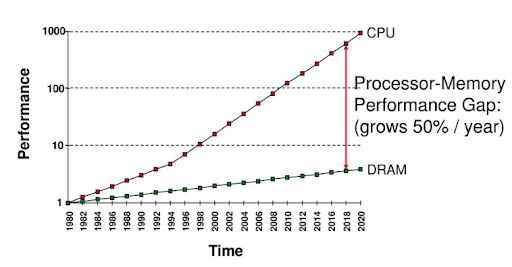
\includegraphics[scale=0.7]{images/gap-processor-memory.png}\\
      \footnotesize{Fonte: \cite{paper-gap-between-processor-memory}}
      \label{fig:processor-memory-performance-gap}
\end{figure} 

Nas arquiteturas computacionais modernas essa hierarquia é formada por: registradores, cache, memória primária e memória secundária. A \figref{fig:hierarquia-de-memoria}  demonstra uma hierarquia de memória, é possível observar que, à medida que nos afastamos do topo da pirâmide, o tempo necessário para concluir uma solicitação do processador à memória (latência) e a capacidade de armazenamento também aumenta.

Devido  a alta latência que as memórias mais distantes do processador possuem, torna-se ideal trabalhar nos níveis superiores da hierarquia de memória para obter um desempenho efetivo das operações sobre um conjunto de dados  \citep{book-compact-data-structures}. A grande problemática é que, conforme disposto por \cite{paper-gap-between-processor-memory}, as memórias com latência menor possuem capacidade de armazenamento também menor, tornando praticamente inviável manipular grandes conjuntos de dados nestes níveis, o que é cada vez mais necessário nos dias atuais, devido ao aumento crescente na produção e consumo de dados. Uma possível solução para tanto é operar sobre os dados em sua forma compactada, e conforme cita também \cite{coira-feranando}, a melhor maneira de fazer isso é através do uso das estruturas de dados sucintas.

\begin{figure}[!ht]
    \centering
    \caption{Hierarquia de memória}
    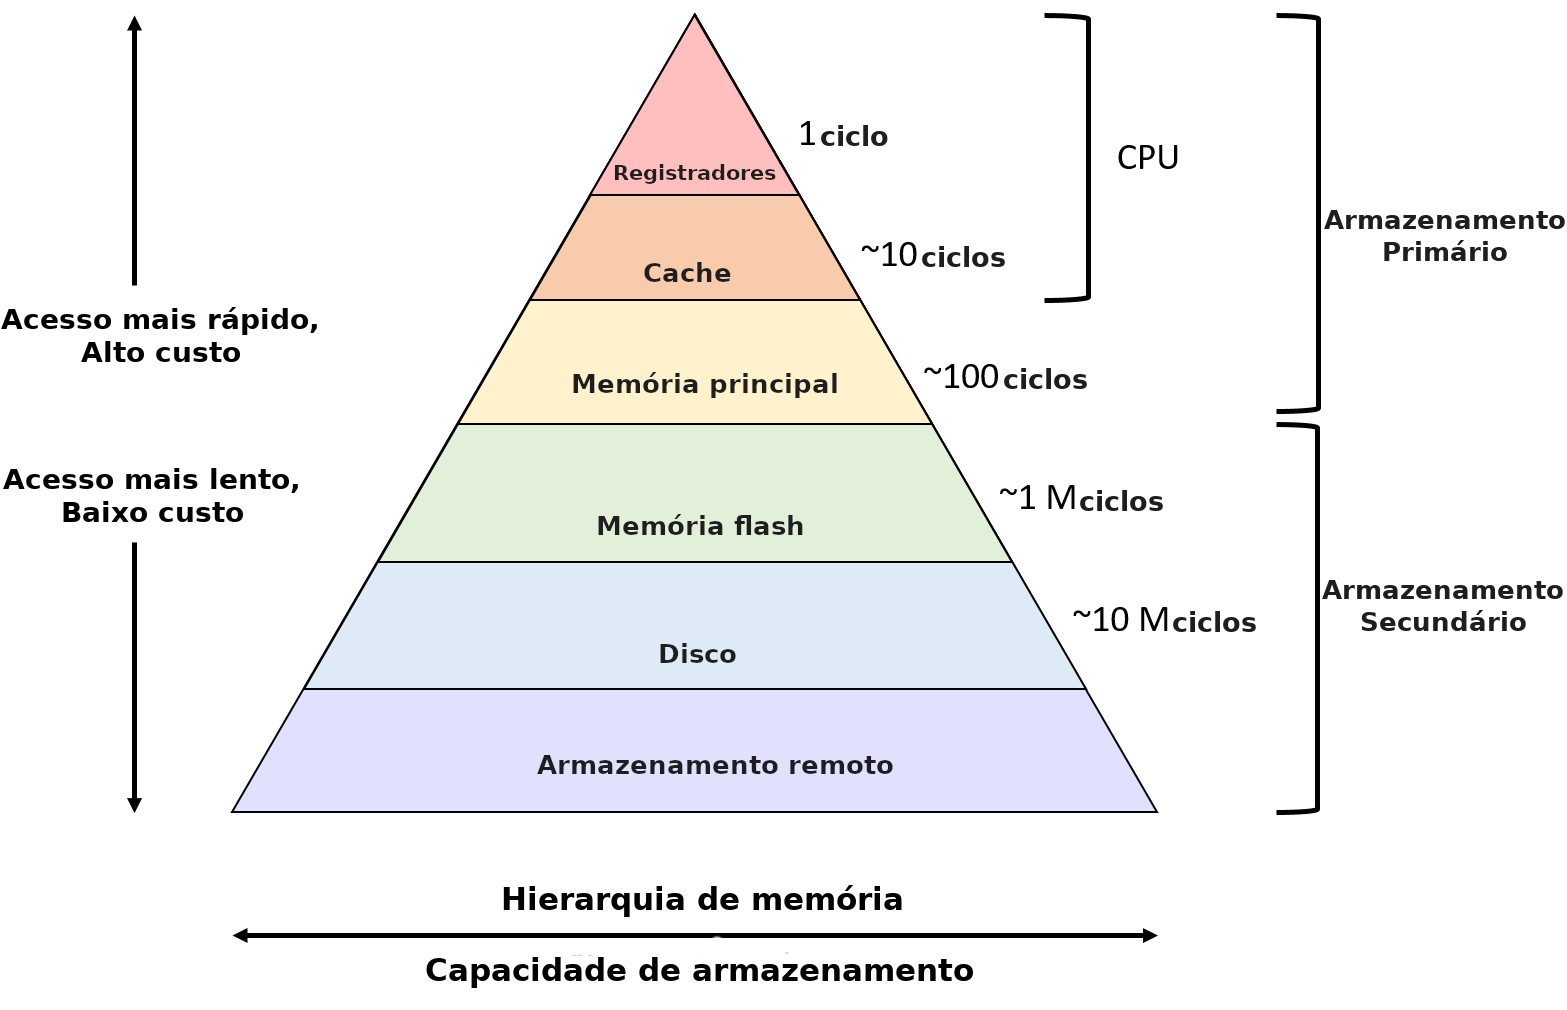
\includegraphics[scale=0.63]{images/hierarquia-memory-2.png}
    \footnotesize{Fonte: \cite{memory-hierarchy}}
  \label{fig:hierarquia-de-memoria}
\end{figure}

Possuindo relação direta com a Teoria da Informação\footnote{Teoria matemática proposta inicialmente por Claude Shannon que busca quantificar a informação.}, uma estrutura de dados é dita sucinta se ela pode representar informações usando um espaço próximo a entropia\footnote{Número mínimo de bits necessários para diferenciar um objeto em um conjunto de dados.} determinada por essa teoria, que como mostra \cite{book-compact-data-structures},  em seu livro, no pior caso é de $\log_2 |U|$ bits para um conjunto de objetos de cardinalidade $U$. Além disso, essa estrutura deve fornecer suporte a uma série de operações primitivas sobre os seus objetos de modo eficiente. Por fim, uma estrutura de dados sucinta é considerada mais eficiente do que outros algoritmos de compactação clássicos, porque estes precisam descompactar os dados a cada operação \citep{coira-feranando}, tornando inviável a manipulação de grandes conjuntos de dados em memórias como a cache e a RAM, ao passo que nas estruturas de dados sucintas, não é necessário descompatar a informação para operar sobre ela.


\section{Árvores Sucintas}
"Sendo uma das estruturas de dados mais difundidas na computação, as árvores também são uma das histórias de sucesso mais marcantes nas estruturas de dados sucintas" \cite[tradução nossa]{book-compact-data-structures}. Uma árvore $T=(V,E)$ é uma estrutura de dados hierárquica, ou seja não linear, formada por vértices (V) e arestas (E). Assim, árvores são definidas também como grafos, sendo eles conexos, não dirigidos e acíclicos, ou seja para qualquer dois vértices em $T$ existe um único e simples caminho \citep{book-algoritmos-teoria-pratica}.



Encontramos diversas aplicações construídas a partir destas estruturas, entre elas, aplicações de banco de dados e tradutores de idiomas \citep{book-algoritmos-teoria-pratica}. Árvores também são amplamente usadas no campo de aprendizagem de máquina: são as chamadas árvores de decisão, que auxiliam desde a escolha do melhor movimento em um jogo de xadrez  à operações em sites de comércio eletrônico \citep{book-inteligencia-artificial}. 
Outra aplicação das árvores no mundo real, se dá através do mapeamento de \textit{Domain Name System (DNS)} em endereços \textit{IP} (e virse-versa). Como mostra  \citep{arvore-dns}  a aŕvore de \textit{DNS} representa de modo hierárquico os nomes de um domínio, facilitando a sua administração e escalonamento. O \textit{DNS} é armazenado de forma invertida na árvore, e cada nó possuí um rótulo (de até $63$ caracteres), representando um \textit{host} ou \textit{subdomínio}, a raíz, por padrão, recebe um rótulo nulo, e o nome de qualquer domínio pode ser obtido a partir do percurso de um nó folha até chegar ao nó raíz.
\begin{figure}[h!]
    \centering
      \caption[Exemplos de representação gráficas de árvores]{Exemplos de representação gráficas de árvores}
      \subfigure[ref1][Árvore de DNS, a subárvore enraízada no nó \textbf{com} define o domínio \textit{data.structure.trees.com}]{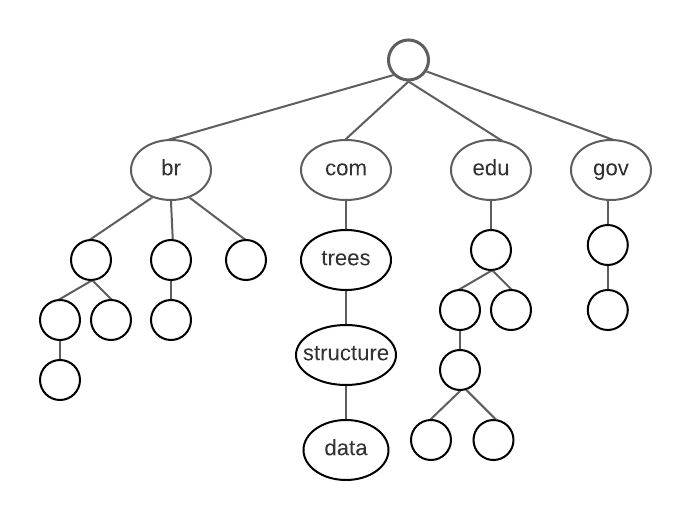
\includegraphics[scale=0.8]{images/tree-dns.png}}
      \qquad
      \subfigure[ref1][Segmento de uma árvore de decisão para um jogo da velha]{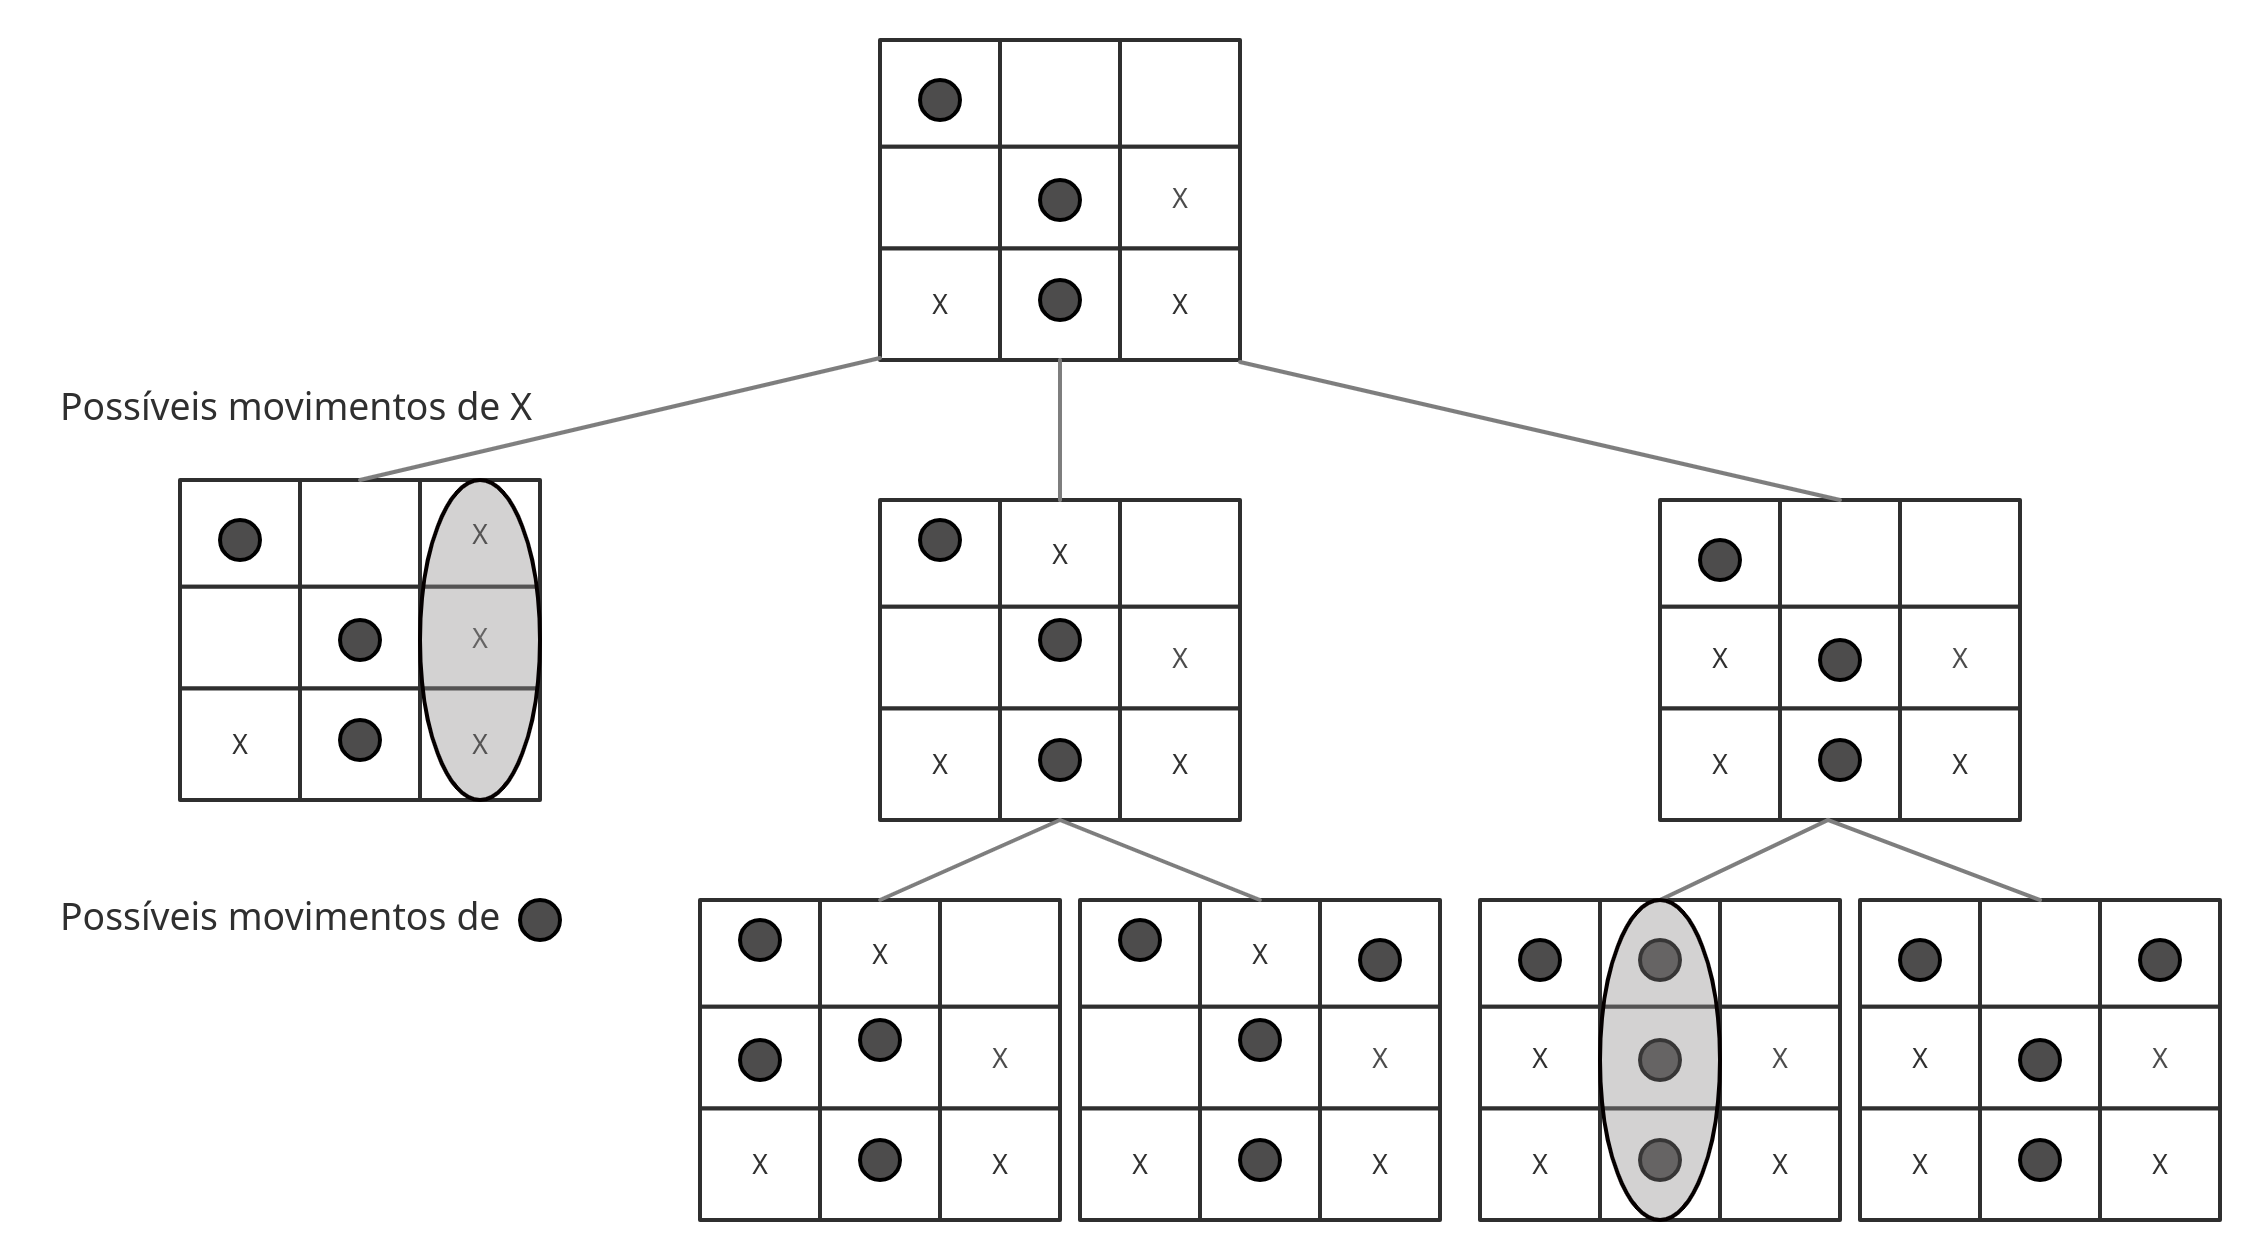
\includegraphics[width=\columnwidth]{images/decision-tree.png}}
      \label{fig:example-tree}
\end{figure}
É possível ver um exemplo de uma árvore de \textit{DNS},  que armazena o domínio \textit{data.structure.trees.com} na \figref{fig:example-tree}, e também uma parte de uma árvore de decisão usada em um jogo da velha.

Mesmo estruturas eficientes como as árvores podem se tornar inviáveis para determinadas aplicações. A forma como estas são construídas afim de operar sobre os objetos podem muitas vezes ocupar um espaço ainda maior do que os dados ocupariam originalmente. Para reconhecer este problema \citet{book-compact-data-structures}, traz como exemplo uma comparação do espaço ocupado pelo genoma humano armazenado sem estruturas adicionais, e o espaço ocupado pelo mesmo usando uma árvore de sufixos que viabiliza operações de montagem de genomas. Com  3,3 bilhões de nucleotídeos, se usarmos 2 bits para armazenar cada base nitrogenada necessitaremos de aproximadamente 825 megabytes, assim podemos reter o DNA por completo em qualquer memória principal. No entanto, usando a árvore de sufixos, cada nucleotídeo precisará de 10 bytes para ser representado, o que nos leva a uma estrutura que ocupa um espaço igual a 33 gigabytes, o que torna inviável o processamento do genoma em memória principal em computadores comuns utilizando esta estrutura de de dados. %Fazendo com que seja necessário armazenar parte do mesmo em memórias como o disco, o que como já vimos acarreta em um alto custo computacional.

É nesse ponto que entram as estruturas de dados sucintas. Como já vimos, estas são capazes de armazenar tanto as informações, como as estruturas de dados que atuam sobre elas usando um espaço reduzido. No caso das árvores que é o objeto do nosso estudo, a sua representação clássica com ponteiros  ocupa  $O(n \log n)$ bits\footnote{Neste trabalho, quando não indicado, estaremos trabalhando com o logarítmo na base 2.}, enquanto existem representações sucintas, abordadas nas Seções \ref{sec:sec-bitvector} e \ref{sec:sec-parenthesis-balanceados}, que ocupam cerca de $2n+o(n)$ bits, conforme disposto em \cite{book-compact-data-structures}.

\section{Vetores de Bits}\label{sec:sec-bitvector}
Um vetor de bits $BV[0,n-1]$  é uma sequência sobre o alfabeto $\Sigma = \{0,1\}$. É possível executar as seguintes operações sobre os vetores de bits \citep{book-compact-data-structures}:

\begin{itemize}
    \item $access(BV,i)$: retorna o $i-$ésimo bit do vetor $BV$, com $0 \leq i < n$;
    \item $rank_v(BV,i)$: seja $v \in \{0,1\}$, e $0 \leq i < n$, esta operação retorna o número de ocorrências de $v$ no intervalo $BV[0,i]$.\\
    Sendo que a seguinte relação de equivalência é válida: $rank_0(BV,i)=i +1  - rank_1(BV,i)$;
    \item $select_v(BV,i)$: dado $v \in \{0,1\}$, com $1 \leq i \leq n_v$, e sendo $n_v$ o número máximo de ocorrências de $v$ em $BV$,
    $select$ retorna a posição do $i-$ésimo bit $v$ em $BV[0,n-1]$.
\end{itemize}

A \figref{fig:bitvector-operations} traz exemplos das operações listadas acima.
\begin{figure}[h!]
\centering
  \caption[Operações sobre vetores de bits]{Operações de $rank, select$ e $access$ sobre $B=111010011000$}
  \subfigure[Operação de $access$ sobre $B=111010011000$][$access(BV,4)=1$]{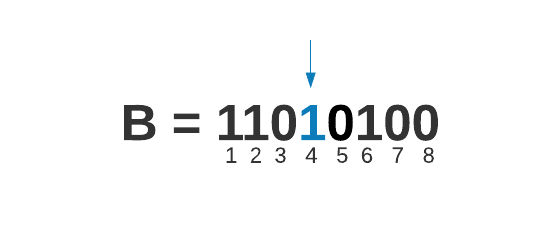
\includegraphics[scale=1.0]{images/access.png}}
  \subfigure[Operação de $rank$ sobre $B=111010011000$][$rank_1(BV,6)=4$]{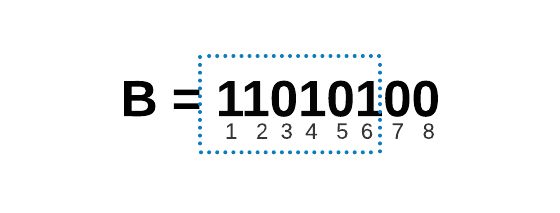
\includegraphics[scale=1.0]{images/rank.png}}
  \subfigure[Operação de $select$ sobre $B=111010011000$][$select_0(BV,6)=8$]{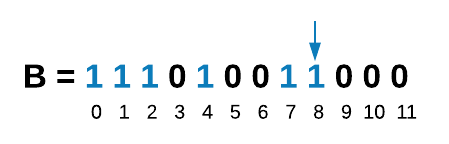
\includegraphics[scale=1.0]{images/select.png}}
  \label{fig:bitvector-operations}
\end{figure}

\section{Representação de árvores sucintas}
Existem diversas formas de representar  uma árvore de maneira sucinta, abaixo listamos algumas destas.

\subsection{Parênteses Balanceados (BP)}\label{sec:sec-parenthesis-balanceados}
\begin{figure}[!ht]
\centering
  \caption[Representação de árvores com parênteses balanceados]{Representação de uma árvore $T$, usando parênteses balanceados: fazendo um percurso pré-ordem em $T$ escrevemos um parênteses de abertura quando um nó é visitado pela primeira vez, e um de fechamento no percurso de volta após atravessar  sua subárvore \citep{paper-succint-representation-of-balanced-parentheses}}
  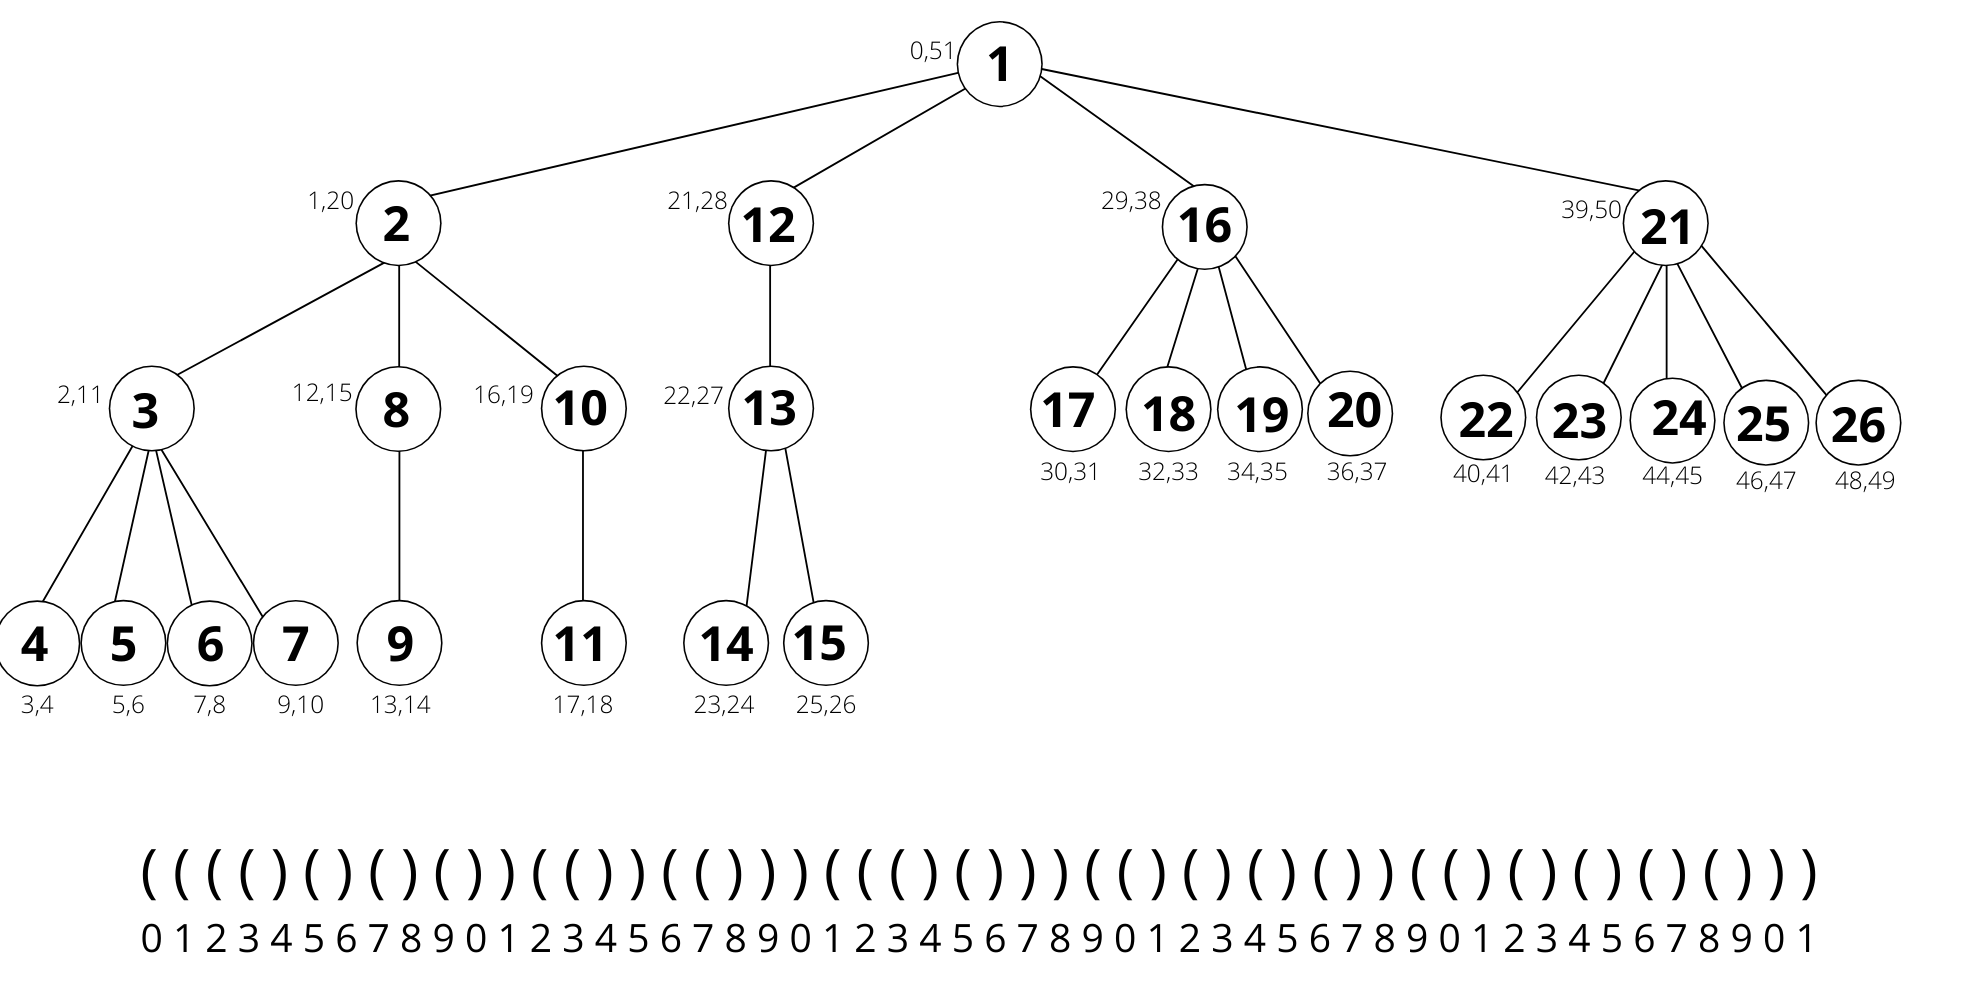
\includegraphics[width=\columnwidth]{images/arvore_geral.png}
  \label{fig:parenthesis-representation}
\end{figure}
Uma sequência de parênteses balanceados (BP) consiste em uma string de tamanho igual a $2n$, sendo $n$ parênteses de abertura '(', e $n$ parênteses de fechamento ')'. Essa estrutura descreve uma relação de hierarquia/contenção, e portanto é amplamente utilizada para a representação de árvores.

Para representar uma árvore ordinária\footnote{Em uma árvore ordinária, cada nó pode ter um número árbitrário de filhos, e as subárvores de cada nó formam um conjunto ordenado de nós \citep{tenenbaum}} $T$ usando essa estrutura, tomamos um vetor de bits de tamanho igual a $2n$ ($BP[0,2n-1])$, em que $n$ é o número de nós da árvore. Realizamos então um percurso sobre $T$ em pré-ordem, e sempre que um nó for alcançado pela primeira vez, um parênteses de abertura (podendo ser representado pelo bit $1$) é inserido em $BP$, ao término da exploração das subárvores deste nó, um parênteses de fechamento (bit $0$) é adicionado em $BP$ \citep{paper-succint-trees-in-practice}.  Na figura \figref{fig:parenthesis-representation} pode-se observar uma árvore com 26 nós e sua representação equivalente em parênteses balanceados.
%Para representar uma árvore ordinal $T$ usando essa estrutura tomamos um vetor de tamanho igual à $2n$ ($BP[0,2n-1])$ onde $n$ é o número de nós da árvore. O nó $v$ (codificado em $BP[i]$) da árvore $T$ é representado por um parênteses de abertura e um de fechamento em $BP$, os elementos contidos no intervalo aberto desses parênteses codificam as subárvores de $v$ em ordem de igual maneira. Na figura \figref{fig:parenthesis-representation} vemos um árvore com 14 nós e sua representação equivalente em parênteses balanceados.

Usando a representação de parênteses balanceados junto à  estruturas de dados auxiliares, podemos fornecer suporte a diversas operações sobre árvores, tais como: \textit{findClose, findOpen} e \textit{excess}. Além dessas três operações, \citet{paper-succint-representation-of-balanced-parentheses} em seu trabalho, traz suporte as operações  \textit{enclose} e \textit{double\_enclose} sobre árvores representadas por intermédio de parênteses balanceados. Estas cinco operações são descritas a seguir:

\begin{itemize}
    \item $findClose(BP,i)$: retorna a posição $j$ do parênteses de fechamento, correspondente ao i-ésimo parênteses de abertura;
    \item $findOpen(BP, i)$: retorna a posição $j$ do parênteses de abertura, correspondente ao i-ésimo parênteses de fechamento;
    \item $excess(BP, i)$: retorna a "diferença entre o número de parênteses abertos e fechados até a posição $i$"  \cite[tradução nossa]{paper-succint-representation-of-balanced-parentheses};
    \item $enclose(BP,i)$: retorna o pai de um nó codificado em $i$;
    \item $double\_enclose(BP,i)$: por sua vez retorna o ancestral comum mais baixo dos nós $i$ e $j$ (operação $lca$).
\end{itemize}
%\citet{paper-succint-representation-of-balanced-parentheses} propuseram uma solução em árvores binárias usando a representação de parênteses balanceados, nesta proposta,  além das operações já citadas, os autores viabilizaram suporte a operação de $enclose(i)$, que retorna o pai de um nó codificado em $i$,  e a operação $double\_enclose(i,j)$ (que equivale à operação $lca$ em árvores) que por sua vez retorna o ancestral comum mais baixo dos nós $i$ e $j$. 

Com base na operação  $rank$, da estrutura de vetores bits, podemos viabilizar a operação de $excess$ facilmente, como mostrado abaixo:

\begin{eqnarray*}
    \begin{split}
        excess(BP,i) &= rank_1(BP,i) - rank_0(BP,i) \\
        &  = rank_1(BP,i) - (i - rank_1(BP,i)) \\
        &  = 2 \cdot rank_1(BP,i) - i -1 
    \end{split}
\end{eqnarray*}

Diversas operações sobre árvores podem ser derivadas de outras operações que usam como base sucessivas computações de excesso dentro de um intervalo. Por exemplo, através de \textit{excess} é possível calcular a profundidade de um nó, isso se deve ao fato de que qualquer nó $x$ é codificado através de um parênteses de abertura, e esse parênteses adiciona um excesso de $1$ unidade à um intervalo iniciado em $i$. A \figref{fig:excess-in-tree} traz a sequência de parênteses balanceados equivalente a árvore da \figref{fig:parenthesis-representation}, e, destaca a área analisada para obter a profundidade do nó $9$ em relação à raíz, neste caso o excesso de parênteses abrindo em relação à quantidade de parênteses fechando é $4$, que é igual a profundidade do nó analisado.

\begin{figure}[!ht]
    \centering
      \caption[Representação de árvores com parênteses balanceados]{Área inspecionada para obter a profundidade do nó $9$ da \figref{fig:parenthesis-representation}}
      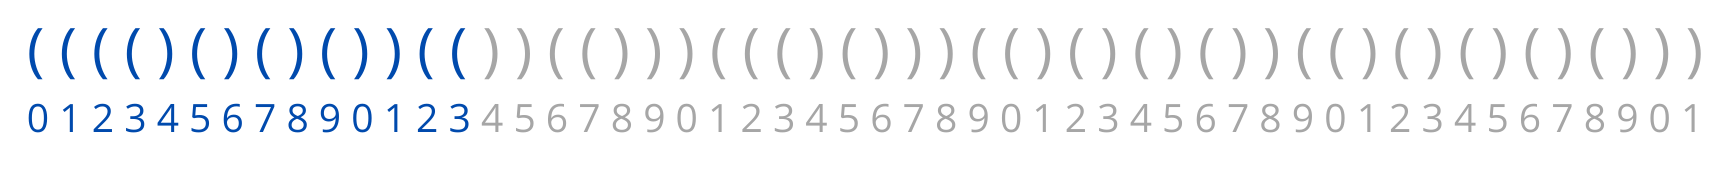
\includegraphics[width=\columnwidth]{images/excess-in-tree.png}
      \label{fig:excess-in-tree}
    \end{figure}

Além de obter a profundidade de um nó, através das operações definidas anteriormente, podemos obter, por exemplo, o tamanho da subárvore de um nó $i$, que pode ser calculada através de: $(findClose(BP,i)+i-1)/2$ (esta expressão retornará a quantidade de nós codificados dentro do intervalo de contenção de $i$). 

Levando em consideração que em $BP$ um nó é codificado através de um parênteses de abertura, podemos responder facilmente se um nó codificado em $j$ é ou não, um nó folha, para tanto, basta averiguar se o elemento que segue o índice $j$, codifica um novo nó, em caso afirmativo, o nó codificado por $j$ possuí filhos, e portanto não pode ser um nó folha, caso o elemento armazezando em $j+1$ corresponda à um parênteses de fechamento significa que o nó $j$ não possuí filhos, e portanto é um nó folha. Esta verificação pode ser feita através da operação de $access(BP,j+1)$.

Por fim, uma das vantagens da \textit{sequência de parênteses balanceados}, como cita \cite{book-compact-data-structures}, é que a mesma permite que qualquer subárvore de um nó seja mapeada de forma contígua em um vetor de bits, o que simplifica uma série de operações existentes sobre árvores.

\subsection{Depth-First Unary Degree Sequence (DFUDS)}
Outra forma de representar árvores é através da \textit{Depth-First Unary Degree Sequence} \citep{article-dfuds}, que assim como em $BP$ faz o uso de uma travessia pré-ordem para construir a árvore à qual representa.
A diferença é que  para codificar um nó, inserimos $i$ parênteses de abertura (onde $i$ é o número de filhos deste nó) e \textit{um} parênteses de fechamento.  Desse modo, o nó passa a ser representado pela posição de seus $i$ parênteses de abertura. A \figref{fig:dfuds-representation}, mostra a representação equivalente à de parênteses balanceados, usando \textit{DFUDS}.
\begin{figure}[!ht]
    \centering
      \caption[Representação de árvores com Sequência de Grau Unário]{Representação de uma árvore $T$ usando DFUDS. O primeiro parênteses (em negrito) não codifica nenhum nó, e foi adicionado ao início da sequência  para torná-la balanceada.}
      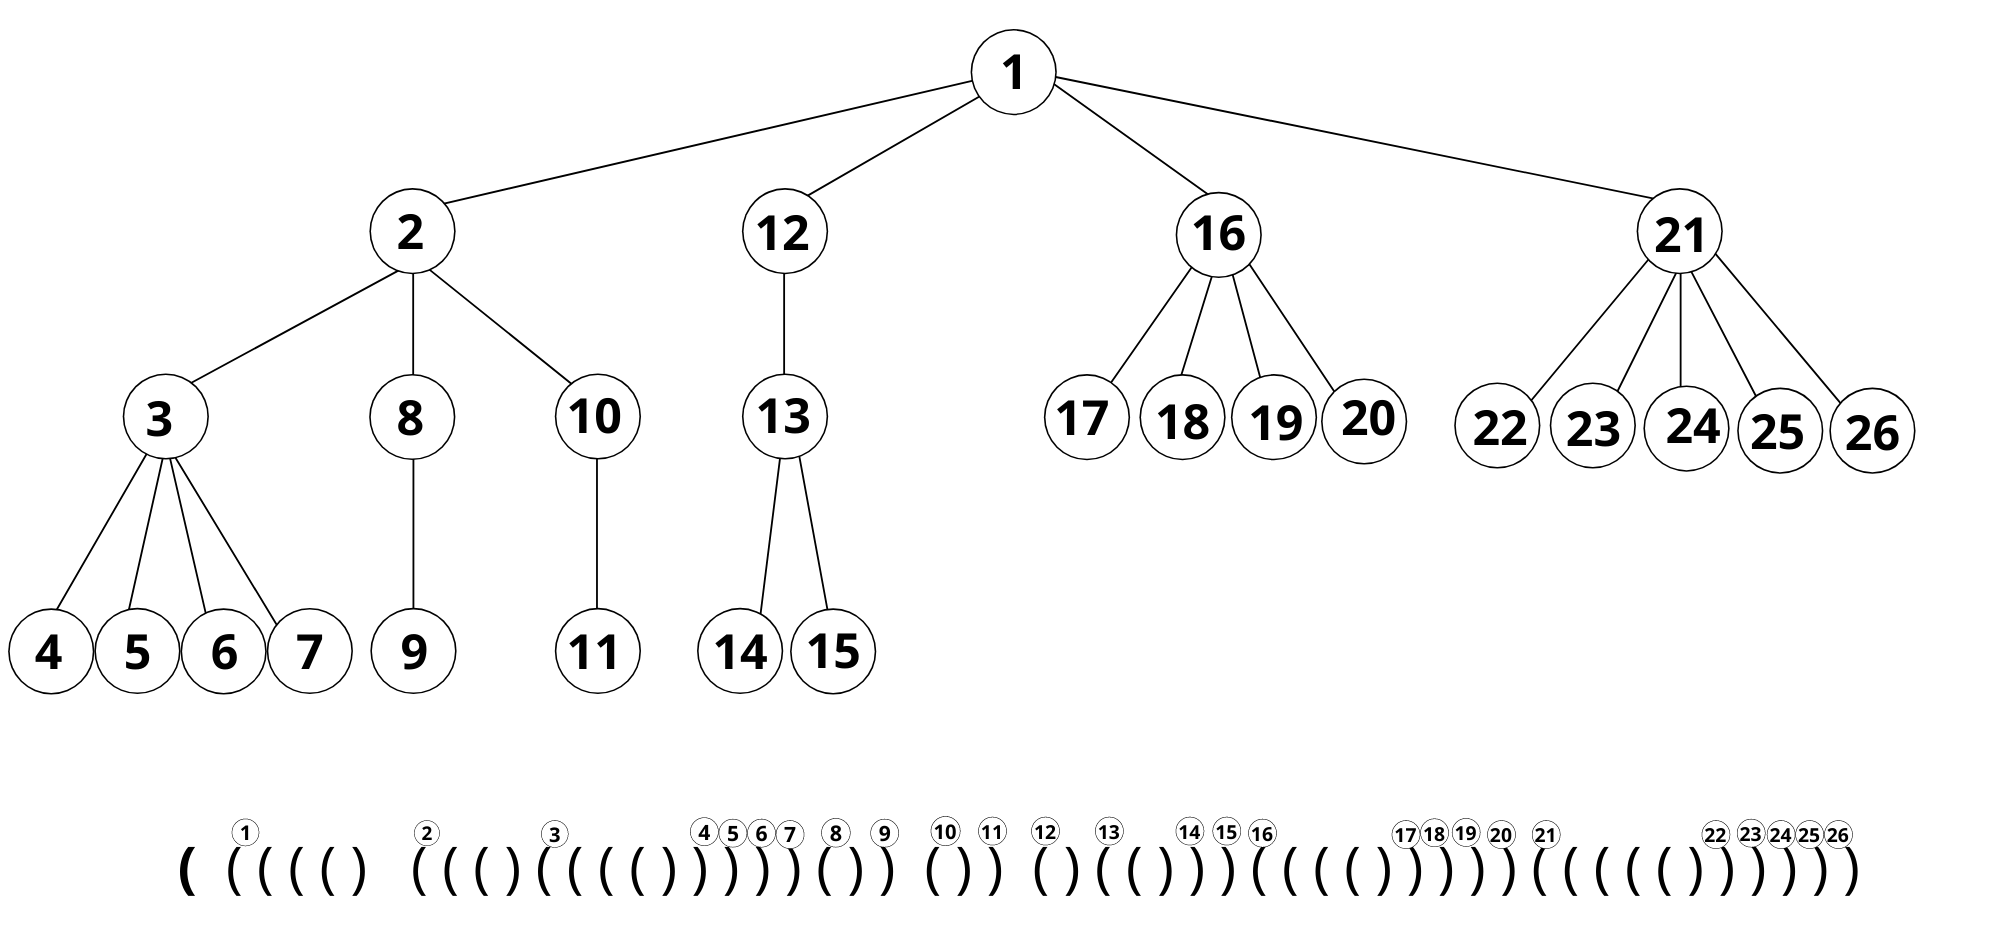
\includegraphics[width=\columnwidth]{images/dfuds.png}
      \label{fig:dfuds-representation}
\end{figure}

Como um nó nessa representação é codificado através do parênteses de abertura (ou bit $1$) de seus $i$ filhos, adicionado de um parênteses fechamento, temos que a sequêrncia gerada em \textit{DFUDS} não é totalmente balanceada, apresentando $n-1$ parênteses de abertura (como sabemos um nó raíz não possuí pai, e portanto, seu parênteses de abertura não é codificado na sequência), e $n$ parênteses de fechamento.  Afim de deixar a sequência balanceada, podemos adicionar um parênteses de abertura ao início da mesma, como é feito em \citet{paper-succint-trees-in-practice}.

\citet{book-compact-data-structures} afirma em seu trabalho, que nessa representação é mais  rápido descer até o $i-$ésimo filho de um nó de uma árvore $T$, pois como a mesma é codificada através de um percurso em pré-ordem, basta avançar  $i$ posições a partir do ínicio da codificação de um nó, no vetor que contém a sequência. Ademais, assim como em $BP$, qualquer subárvore de um nó, é mapeada de modo contíguo em um vetor, entretanto, a área dessa subárvore não pode ser delimitada por um parênteses de fechamento, como acontece para \textit{parênteses balanceados} \citep{book-compact-data-structures}.

\subsection{Level-order Unary Degree Sequence (LOUDS)}
\begin{figure}[h!]
    \centering
      \caption[Representação de árvores com Level-order Unary Degree Sequence]{Representação de uma árvore $T$ usando LOUDS. 
      Assim como em DFUDS foi adicionado de um parênteses de abertura no início da sequência  para que a mesma se tornasse balanceada.}
      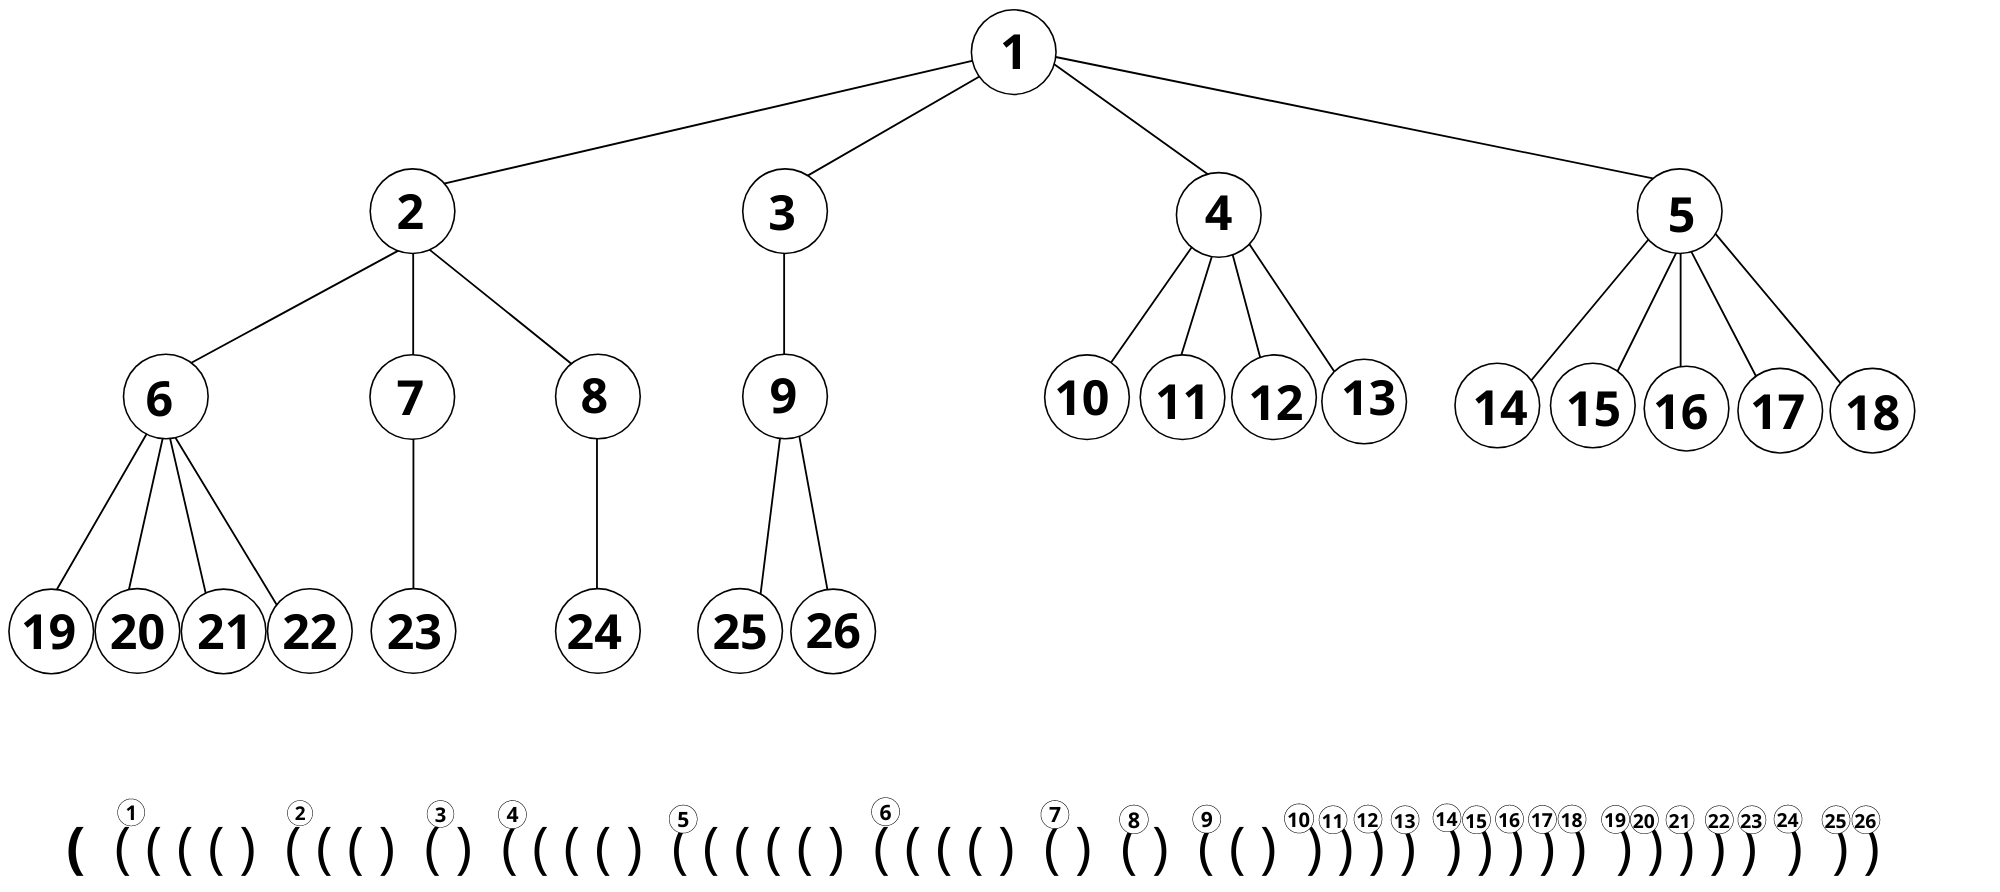
\includegraphics[width=\columnwidth]{images/louds.png}
      \label{fig:louds-representation}
\end{figure}
Na representação \textit{Level-order Unary Degree Sequence} \citep{article-louds,article-dfuds} pecorremos os nós da árvore por meio de um percurso em largura, adicionando assim como em \textit{DFUDS}, $i$ (novamente com $i$ representando o grau do nó) parênteses de abertura ao visitarmos um nó pela primeira vez, seguido de um parênteses de fechamento.
 Devido ao percurso utilizado para codificar a árvore nesta representação, as subárvores de um nó não são mapeadas de forma contígua no vetor que a representa, inviabilizando operações básicas como o cálculo do tamanho da subárvore de um nó \citep{book-compact-data-structures,paper-fully-functinal-succint-trees}.

A \figref{fig:louds-representation} mostra uma representação em \textit{LOUDS} para a árvore $T$, usada como exemplo na representação de \textit{parênteses balanceados} e em \textit{DFUDS}.

\section{Range min-Max Tree (rmM-tree)}\label{sec:sec-classic-rmm-tree}
Proposta por \citet{paper-fully-functinal-succint-trees}, estudada por diversos outros autores, a range min-Max tree, é uma estrutura baseada em valores de excessos máximos e mínimos dentro de um intervalo. 

A rmM-tree viabiliza a realização de operações de percurso e busca (além das definidas na Seção~\ref{sec:sec-parenthesis-balanceados}) sobre árvores codificadas por meio de sequências de parênteses balanceados. O uso da estrutura de parênteses balanceados implica na redução de um grande número de operações relevantes consideradas na literatura a poucas operações primitivas, podendo estas serem realizadas em tempo constante para árvores suficientemente pequenas \citep{paper-fully-functinal-succint-trees}.

Neste trabalho usaremos a abordagem mostrada por \citet{book-compact-data-structures} em seu livro, para a construção da rmM-tree binária. Como explica o autor, a range min-Max tree é construída na forma de uma árvore binária completa --o que nos permite a utilização de vetores, omitindo o uso de ponteiros explícitos -- sendo que cada um de seus nós armazena os valores de excesso calculados dentro de um intervalo do vetor que representa a árvore de entrada. 

A construção da rmM-tree segue uma abordagem \textit{bottom-up}, onde para cada nó, calcula-se primeiro o intervalo a ser coberto, para então definirmos os  valores de excesso. Após construir os nós folhas dessa estrutura, repetimos o processo descrito para os nós internos (e raíz), sendo que o intervalo coberto por cada nó não folha é dado pela união da área coberta pelos seus nós filhos.

%A quantidade de intervalos armazenados por essa estrutura influência diretamente na complexidade de espaço ocupado pela mesma. 
Como cada nó folha de uma rmM-tree está associado a um único intervalo, o tamanho de uma rmM-tree está também relacionado a quantidade e ao tamanho dos intervalos cobertos pela mesma. 
Esses intervalos são obtidos da seguinte maneira: dado um vetor de entrada $BP$, de  tamanho igual a $n$, sendo $BP$ usado para a codificação via parênteses balanceados de uma árvore $T$ com tamanho igual a $n/2$, é definido um tamanho de intervalo $b$ (chamado também de tamanho de bloco), divide-se então $n$ por $b$, obtendo assim a quantidade de folhas da rmM-tree.

Considerando que a altura de uma árvore binária é dada por $\lceil \log n \rceil$ e que o vetor de entrada $BP$ ocupa $n$ bits, temos assim que a rmM-tree utiliza um espaço próximo a $n + O(\frac{n}{b} \log n)$ bits. Tomando $b = \log^2 n$, temos uma complexidade de espaço a $n + O(n/\log n)$. Em relação ao tempo gasto por cada operação sobre a rmM-tree,  \citet{book-compact-data-structures} mostra que na prática todas essas operações podem ser realizadas em tempo $O(\log n)$ - ou ainda em tempo $O(\log \log n)$ em uma versão mais refinada da estrutura - a lista completa dessas operações é apresentada na \tabref{tbl:classicOperations-rmm-tree} deste capítulo.


\subsection{Registros}
Os valores de excesso definidos em cada nó da rmM-tree são essenciais para a realização de operações de consulta de maneira eficiente, são neles em que essa estrutura se baseia.  Em seu livro, \citet{book-compact-data-structures}, define 4 valores de excesso que viabilizam essas operações. Mostraremos as definições de cada um destes a seguir. 

Suponha que um nó $v$ cubra um intervalo $[s,e]$ do vetor de entrada $BP$ definido anteriormente, então:
\begin{itemize}
    \item \textit{R[v].e}: armazena o excesso total no intervalo $[s,e]$.
    
    $R[v].e = excess(e) - excess(s-1)$.
    \item \textit{R[v].m}: corresponde ao excesso mínimo local.
    
    $R[v].m = \min\{excess(i) - excess(s - 1) | s \leq i \leq e\}$.
    \item \textit{R[v].M}: corresponde ao excesso máximo local.
    
    $R[v].M = \max\{excess(i) - excess(s - 1) | s \leq i \leq e\}$.
    
    \item \textit{R[v].n}: é definido pelo número de vezes que o excesso mínimo ocorre dentro do intervalo coberto. Assim, suponha $m$ o valor do excesso mínimo no intervalo $[s,e]$, então:

    $R[v].n = |\{s \leq i \leq e | excess(i) = R[v].m\}|$
    %$R[v].n= |{p \in BP[s,e], excess(p) - excess(s - 1) = R[v].m}|$
\end{itemize}

    Agora que temos a definição de cada registro da range min-Max tree, podemos construir os nós folhas da nossa estrutura, e os demais nós nível a nível, partindo das folhas. Os nós internos e raíz da nossa árvore, são calculados a partir dos valores de seus nós filhos. Como a nossa estrutura é construída usando um vetor, podemos navegar até os filhos de um nó $v$ através de aritmética básica nos índices da nossa árvore, desse modo, o filho esquerdo de um nó $v$ é dado por $(2 \cdot v)+1$, ao passo que o filho direito desse nó pode ser obtido a partir de $(2 \cdot v) +2$. Essa relação entre os valores dos registros de um nó pai e um nó filho, é descrita pelas equações abaixo:

    \begin{itemize}
        \item $R[v].e = R[2v +1 ].e + R[2v + 2].e$
        \item $R[v].m = min(R[2v+1].m, R[2v+1].e + R[2v + 2].m)$
        \item $R[v].M = max(R[2v+1].M, R[2v+1].e + R[2v + 2].M)$
        \item $ R[v].n =
           \begin{cases}
                 R[2v+1].n, & \mbox{se } R[2v+1].m < R[2v+1].e + R[2v + 2].m; \\
                 R[2v + 2].n, & \mbox{se } R[2v+1].m > R[2v+1].e + R[2v + 2].m; \\
                 R[2v+1].n + R[2v + 2].n, & \mbox{se }  R[2v+1].m = R[2v+1].e + R[2v + 2].m .
           \end{cases}
        $
    \end{itemize}

\begin{example}\label{ex-build-tree}
    Para melhor elucidar a construção dessa estrutura usaremos o exemplo da Seção~\ref{sec:sec-parenthesis-balanceados} e demonstraremos o cálculo dos registros e dos intervalo de um nó folha, mostraremos também como é construído um dos nós internos da rmM-tree. No exemplo em questão, temos um vetor de entrada com 52 parênteses balanceados, e um tamanho de bloco $b = 4$ o que implica que a árvore terá:

    \begin{itemize}
        \item $r = n/b \to r = 52/4 = 13 $ folhas;
        \item 12 nós internos, pois $r-1 = 12$;
        \item Altura $h= \ceil{\log r} \to h = \ceil{\log 13}= 4$;
        \item Como o número de folhas não é uma potência de 2, temos que as folhas $0$ até $2 \cdot r - 2^h  -1 = 9$ estão agrupadas no último nível da árvore,  e as outras $2^h - r = 3$ folhas estão agrupadas à direita no nível anterior.
    \end{itemize}

    Assim temos os seguintes valores de excesso para a folha $0$ (nó $15$) da rmM-tree:
        \begin{itemize}
            \item  Área de cobertura:
            $ BP[0,3]$
            \item Excesso local:
            $R[15].e = excess(3) = 2 \cdot rank_1(BP,3) - 3 - 1= 4$
            \item Excesso mínimo:
            $R[15].m = min(1,2,3,4) = 1$
            \item Excesso máximo:
            $R[15].M = max(1,2,3,4) = 4$
            \item Número de vezes que o excesso mínimo ocorre no intervalo:\\
            $R[15].n = count(1,2,3,4) = 1$
        \end{itemize}
        
    Mostraremos agora o cálculo do 7º nó interno do nosso exemplo, este cobre as folhas 0 e 1 da árvore (nós 15 e 16, respectivamente), com base nas definições anteriores temos então:
    \begin{itemize}
        \item Área de cobertura: $BP[0,3] \cup BP[4,7]$
        \item Excesso global: \\
        $R[7] = R[15].e + R[16].e = 4 + 0 = 4$
        \item Excesso mínimo:\\
        $R[7].m = min(R[15].m, R[15].e+R[16].m) = (1,4-1)=1$
        \item Excesso máximo:\\
        $R[7].M = max(R[15].M, R[15].e+R[16].M) = (4,4+0)=4$
        \item Número de vezes que o excesso mínimo ocorre no intervalo:\\
        $R[7].n = R[15].n = 1$,  pois $R[15].m < R[15].e+R[16].m$
    \end{itemize}

    O processo mostrado acima deve ser repetido para os demais nós da árvore até que cheguemos a raíz, dando origem a árvore mostrada na \figref{fig:rmm-tree-binaria}. 
    \begin{figure}[!ht]
     \centering
      \caption[rmM-tree clássica.]{rmM-tree clássica,com tamanho de bloco igual a 4. A estrutura foi construída a partir dos 52 parênteses balanceados mostrados na parte inferior}
      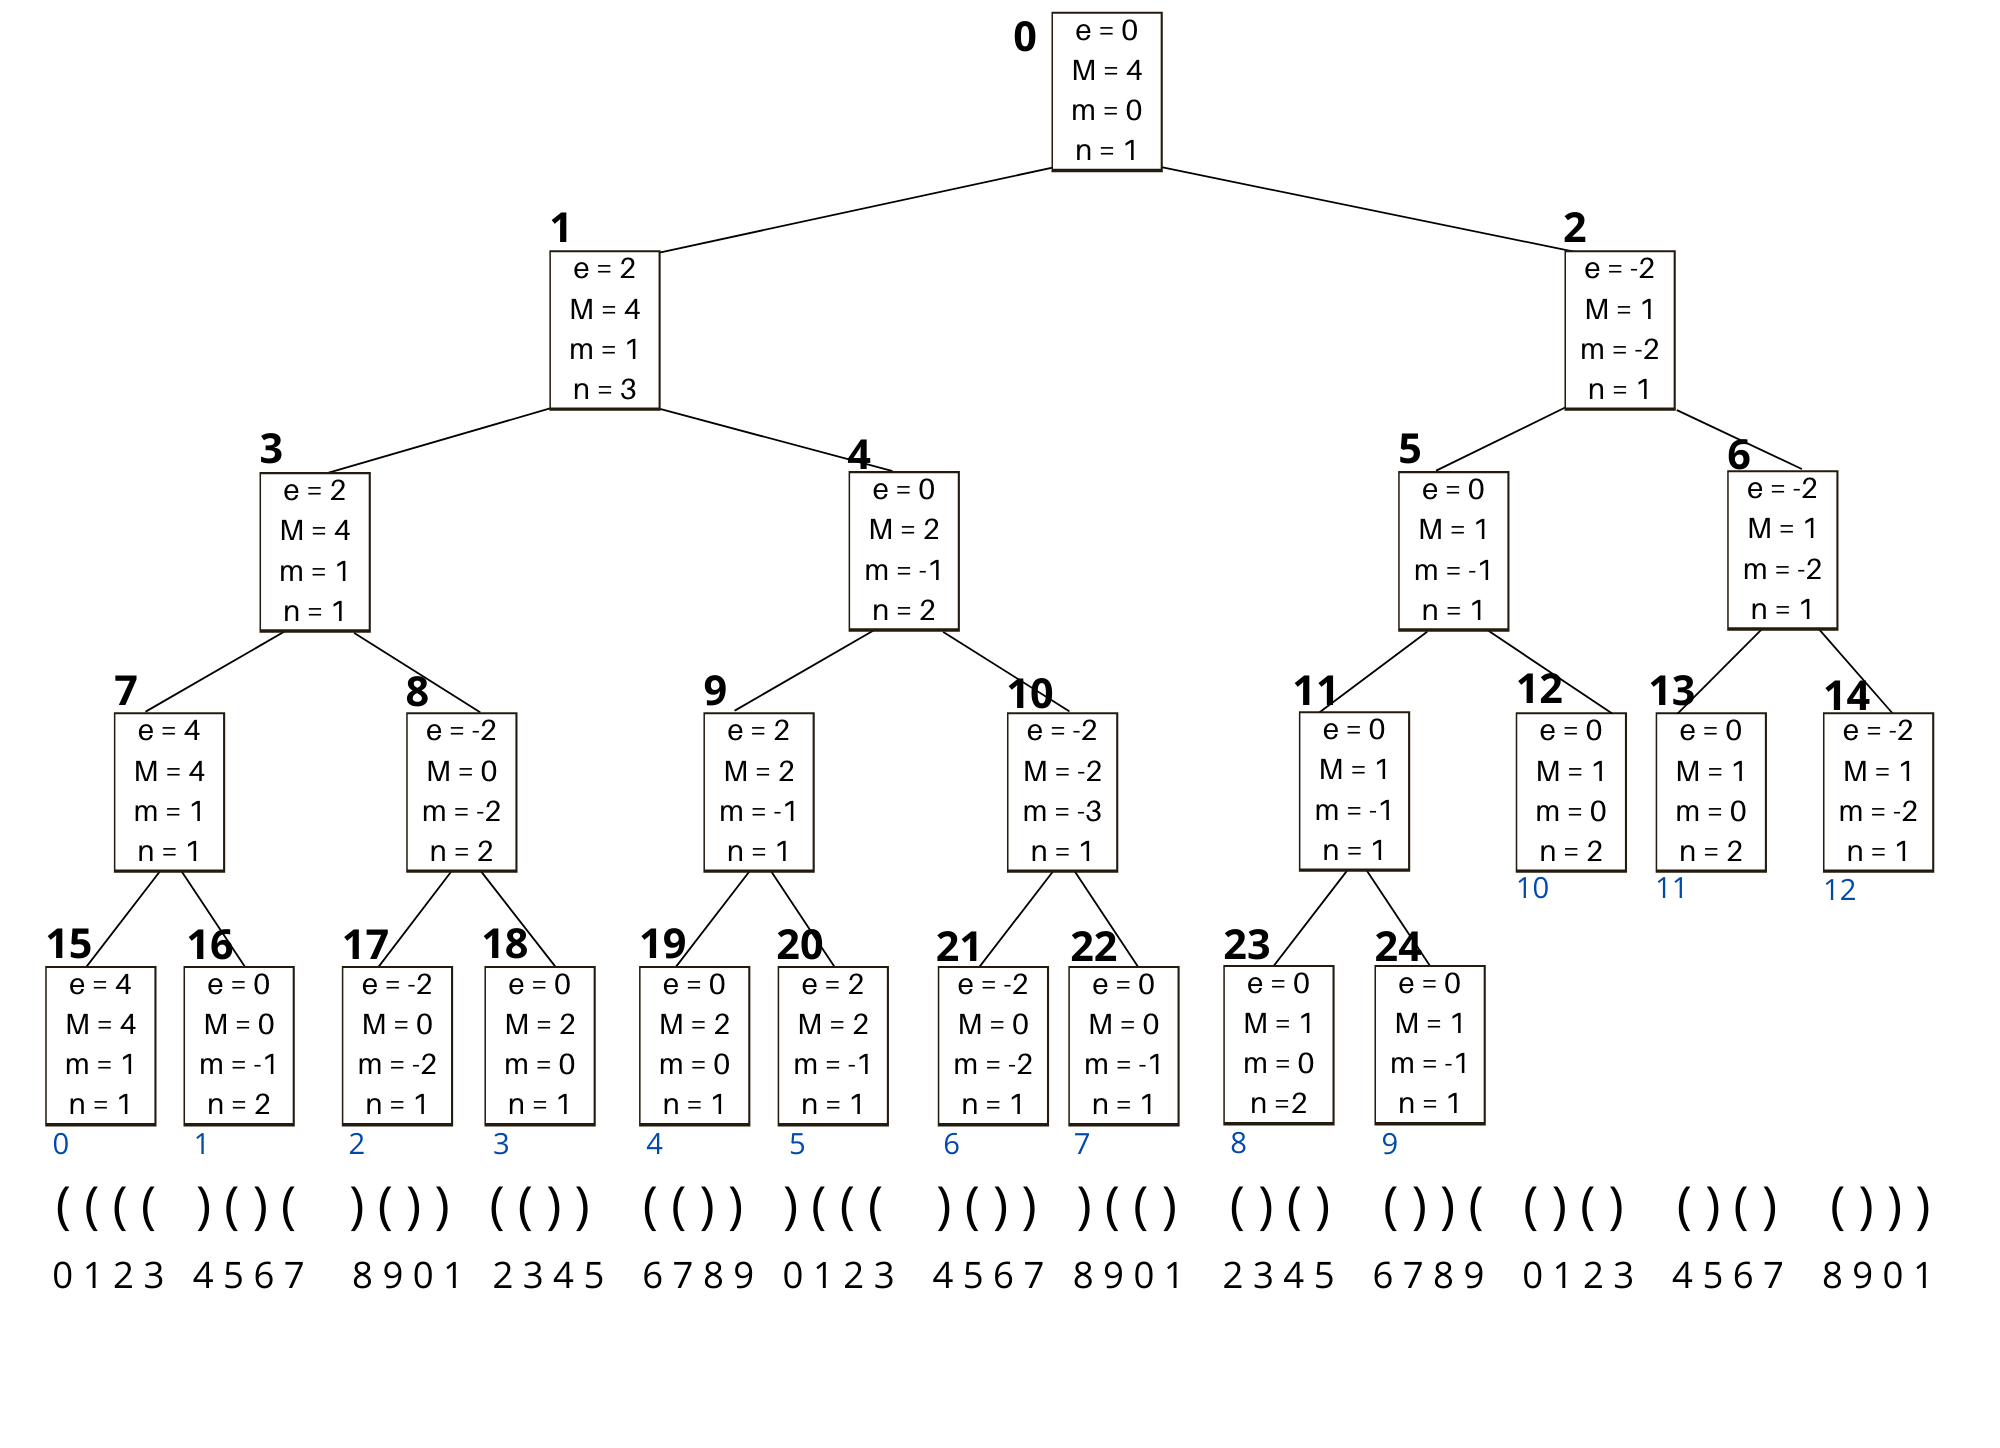
\includegraphics[width=\columnwidth]{images/rmm-tree-bin.png}
      \label{fig:rmm-tree-binaria}
    \end{figure}
\end{example}

O processo de construção da rmM-tree é mostrado com mais detalhes no Algoritmo~\ref{alg:build-bin-tree}. Neste algoritmo, fazemos o uso de uma tabela $C$, esta tabela pré-computa todas as possibilidades de valores de registro para um intervalo de tamanho $w$, sendo $b \mbox{ mod } w = 0$. "Essa técnica de pré-computar todos os valores possíveis de determinados padrões de bits é conhecida como \textit{truque dos quatro russos}" \citep[tradução nossa]{book-gusfield}.
O uso dessa tabela $C$ não é obrigatório para a construção da rmM-tree, entretanto, a mesma possibilita a otimização do tempo de construção e operações sobre a rmM-tree, como disposto em \citet{book-compact-data-structures}.


Conforme expõe \citet{book-compact-data-structures}, a tabela $C$ é construída em tempo $O(\sqrt{n} \log n)$ e ocupa $O(\sqrt{n} w)$ bits de espaço. Esse processo de construção é feito do seguinte modo: após definir uma constante $w$, criamos uma tabela $C[0, 2^w-1]$,  onde cada entrada da tabela armazena os registros de excesso definidos anteriormente, cada elemento $C[x]$ é calculado com base nos $w$ bits  que formam $x$. Para melhor elucidar estre processo, o exemplo abaixo mostra a computação de uma entrada específica da tabela $C$. O Exemplo 3 traz a aplicação da tabela $C$ em um nó da rmM-tree da \figref{fig:rmm-tree-binaria}.
\begin{example}
    Suponha $w=4$ e $x=3$, temos assim que:

    $$3_2 = 0011,$$  logo iterando sobre os bits que formam o número temos os seguintes valores de  registro:
    \begin{itemize}
        \item $C[x].e = 0; C[x].M = 0; C[x].m = -2; C[x].n = 1$
    \end{itemize}
\end{example}

Fazer a pré-computação dessa tabela elimina a necessidade de computar iterativamente os valores de excesso mínimo e máximo, a cada inspeção de bits. Assim, no momento da construção dos nós da rmM-tree, ou durante a inspeção dos mesmos, basta ler os $w$ bits que queremos inspecionar, e então realizar uma consulta na tabela $C$ pelo elemento $x$ que mapeia os bits lidos. Conforme mostra \citet{book-compact-data-structures} uma consulta na tabela $C$ leva tempo constante, já a construção dos nós folhas usando essa técnica leva tempo $O(\frac{n}{\log n})$. Outra operação que atua junto à tabela $C$ é a função \textit{bitsread}, ela recebe como parâmetro um índice $i$, e então lê a palavra formada em $BP$, a partir de $i$, seguido pelos $w-1$ bits após $i$, usando como critério de leitura o bit mais significativo (\textit{Most Significant Bit (MSB)}), após esse processo o valor obtido por \textit{bitsread} é usado para consultar a tabela $C$, em busca dos valores de registro correspondentes aos bits analisados. 

Além da tabela $C$ e da função \textit{bitsRead}, em nossa implementação usamos outras duas funções que nos auxiliam no  percurso em árvore, denominadas \textit{leafInTree} e \textit{numLeaf}, a primeira retorna o índice de um nó na rmM-tree correspondente ao número de uma folha,  a segunda por sua vez retorna o número de uma folha correspondente à um nó da rmM-tree (veja Algoritmo~\ref{alg:folha-indice}). Essas operações são úteis para iniciar (ou finalizar) o percurso na rmM-tree com base em um intervalo específico.


\begin{example}
    Tome como base agora, a nossa rmM-tree de exemplo, assuma $w=4$. Para melhor exemplificação, vamos alterar um pouco a estrutura da nossa árvore, assuma um tamanho de bloco  $b=8$, para este exemplo. Suponha que queremos construir a folha de número $0$ (como aumentamos a cobertura do nosso bloco, a folha $0$, neste exemplo, corresponde à união dos nós $15$ e $16$ da árvore mostrada na \figref{fig:rmm-tree-binaria}), que neste exemplo corresponde ao nó $7$. O intervalo coberto por essa folha vai de $0$ à $7$, assim precisaríamos ler os $8$ bits que compõem esse intervalo. 
    
    Para um exemplo pequeno como  este não há problemas em calcular esses valores iterativamente, mas imagine o que acontece com casos em que temos uma árvore de entrada maior, e tamanho de  bloco também maior, o processo se tornaria mais oneroso. Observe então como este processo é feito usando a tabela de excessos $C$.


    \begin{itemize}
        \item Como $w=4$, convertemos primeiro os bits codificados em $BP[0,3]$\\
        $BP[0,1,2,3] = 1111_2$\\
        Fazemos então uma busca na tabela $C$ pelo elemento $x = 1111_2$, que com base na explicação anterior, traz os seguintes valores:
        $$C[1111_2].e = 4; C[1111_2].M = 4; C[1111_2].m = 1; C[1111_2].n=1.$$
        Nesse momento, os valores do registro da nossa folha são:\\
        $$R[7].e = 4; R[7].M = 4; R[7].m = 1; R[7].n=1.$$
        \item  Agora precisamos computar os valores correspondentes aos $w$ bits restantes que compõem a nossa folha, temos que:
        $BP[4,5,6,7] = 0101_2$. Os registros armazenados em $C$, para este elemento são:
        $$C[0101_2].e = 0; C[0101_2].M = 0; C[0101_2].m = -1; C[0101_2].n=2.$$

        Agora que temos os valores de excesso para cada subintervalo da nossa folha, podemos obter os valores de registro para o intervalo completo, esse processo é similar ao definido para a obtenção dos registros de um nó pai. Temos assim que:
        \begin{itemize}
            \item $R[7].e = R[7].e + C[0101_2].e = 4 + 0 = 4$
            \item $R[7].M = max(R[7].M, R[7].e + C[0101_2].M) =  max(4,4+0) =4$
            \item $R[7].m = min(R[7].m, R[7].e + C[0101_2].m) = min(1,4-1) = 1$
            \item $R[7].n=1,$ pois o excesso mínimo ocorre no primeiro subintervalo da folha.
        \end{itemize}
    \end{itemize}

    Ao observar o nó $7$ do exemplo~\ref{ex-build-tree}, é possível notar, que de fato, os valores obtidos nestes exemplo correspondem ao nó citado.
\end{example}

\newpage

\begin{algorithm}[h!]
    \SetAlgoLined\DontPrintSemicolon
    \SetKwFunction{algo}{algo}\SetKwFunction{proc}{proc}
    \SetKwProg{myproc}{Proc}{}{}
    \myproc{numLeaf(v)}{
        \Input{Índice $(v)$ da rmM-tree.}
        \Output{Número $(l)$ da folha codificada em $R[v]$.}
        \If{$v \geq 2^h-1$}{\Return{$v - 2^h + 1 $}}
        \Else{\Return{$v - 2^h + r + 1$}}
    }

    \setcounter{AlgoLine}{0}

    \SetKwProg{myproc}{Proc}{}{ }
    \myproc{leafInTree(l)}{
        \Input{Número $(l)$ de uma folha na rmM-tree.}
        \Output{Índice $(v)$ onde a folha é codificada na rmM-tree.}
        \If{$l < (2r - 2^h)$}{\Return{$2^h - 1 + l$}}
        \Else{\Return{$2^h - 1 - r + l$}}
    }
    \caption{Conversão entre números de folhas e índice das folhas da rmM-tree.}
    \label{alg:folha-indice}
\end{algorithm}

\begin{algorithm}[h!]
    \SetKwFunction{algo}{algo}
    \SetKwProg{myalg}{Algoritmo}{}{}
    \myalg{buildingTree(BP, C, b, w, r, nNodes)}{
        \Input{Vetor de bits, tabela de excessos C, tamanho de bloco e de subbloco, número de folhas e quantidade de nós. }

        \tcp{Construção dos nós folhas}
        \For{$l \leftarrow 0$ \textbf{to} $r-1$}{
            $v \leftarrow leafInTree(l)$\tcp{Algoritmo~\ref{alg:folha-indice}}
            $(R[v].e, R[v].M, R[v].m, R[v].n) \gets(0,-w,w,0)$\\
            \For{$p \leftarrow (l \cdot (b/w))+1$ \textbf{to} $((l+1) \cdot b)/w$}{
                $x \leftarrow bistread((p-1)\cdot w)$\\
                \If{$R[v].e + C[x].M > R[v].M$}{$R[v].M \leftarrow R[v].e + C[x].M$}
                \If{$R[v].e + C[x].m < R[v].m$}{
                    $R[v].m \leftarrow R[v].e + C[x].m$\\
                    $R[v].n \leftarrow 1$
                }
                \ElseIf{$R[v].e + C[x].m = R[v].m$}{$R[v].n \leftarrow R[v].n + C[x].n$}
                $R[v].e \leftarrow R[v].e + C[x].e$
            }
        }

        \tcp{Construção dos nós internos e raíz}
        \For{$v \leftarrow nNodes - r -1 $ \textbf{to} $0$}{
            $v_l \leftarrow (2 \cdot v)+1$\\
            $v_r \leftarrow v_l + 1$\\
            $R[v].e \leftarrow R[v_l].e + R[v_r].e$\\
            $R[v].M \leftarrow max(R[v_l].M, R[v_l].e + R[v_r].M)$\\
            $R[v].m \leftarrow min(R[v_l].m, R[v_l].e + R[v_r].m)$\\
            \If{$R[v_l].m > R[v_l].e + R[v_r].m$}{$R[v].n \leftarrow R[v_r].n$}
            \Else{ $R[v].n \leftarrow R[v_l].n + R[v_r].n$}
        }
    }
    \caption{Construção da range min-Max tree binária}
    \label{alg:build-bin-tree}
\end{algorithm}


\newpage


\subsection{Operações}
As operações sobre a range min-Max tree são realizadas através de cálculos usando os valores de excesso definidos na seção anterior.  Parte dessas já foram descritas nas Seções \ref{sec:sec-bitvector} e \ref{sec:sec-parenthesis-balanceados}, como as operações  \textit{enclose, findClose  e  findOpen}, nesta seção veremos como computá-las usando os nós da rmM-tree.
Além das operações citadas, existem outras importantes operações suportadas pela range min-Max tree, detalhamos algumas logo abaixo. 

A Tabela~\ref{tbl:classicOperations-rmm-tree} mostra a lista completa das operações suportadas pela range min-Max tree binária.

\subsection{FwdSearch}\label{sec:fwdsearch-bin}
    O objetivo da operação \textit{forward search} (busca à frente), é encontrar um excesso relativo $d$, em relação à um nó codificado em um índice $i$ no vetor que representa uma árvore. Desse modo, \textit{ fwdSearch} retorna um índice $j>i$, mais à esquerda possível, tal que, o nó definido por $j$ está à uma profundidade $d$ em relação ao nó codificado por $i$. O resultado dessa operação é dado pela expressão abaixo:
    $$fwdsearch(i,d) = min\{j > i | excess(j) = excess(i) + d\}$$
    
    Como veremos mais tarde, dessa operação deriva-se diversas outras, tais como \textit{findClose, lca (ancestral comum mais baixo)} e outras operações de percurso em árvore.

    \citet{paper-simple-and-efficient-fully-functional-succinct-trees} descrevem o funcionamento dessa operação da seguinte maneira: dado um excesso desejado $d$, e um índice $i$, a partir do qual a busca dever ser feita, examinamos a folha $k$ (com $k= \floor{(i+1)/b}$), cujo o intervalo de cobertura engloba o índice $i+1$.
    Caso não encontremos $d$ dentro desse intervalo, usamos os nós da rmM-tree para encontrar o bloco a qual $d$ pertence. Avançamos na rmM-tree pelo pai do nó folha analisado, verificando a cada iteração, se o valor do excesso buscado está compreendido no intervalo dos valores de excesso do nó à direita do atual. Ao encontramos o nó que contém o valor de excesso buscado, encerramos o processo de subida na árvore, e iniciamos o processo de descida na rmM-tree até que cheguemos à um nó folha. Durante o percurso de descida, avançamos pelo filho à esquerda do nó corrente sempre que $d$ estiver incluso nos intervalos de contenção do mesmo, e pelo nó à direita caso contrário. Ao chegarmos em um nó folha da árvore, interrompemos a inspeção dos nós da rmM-tree e iniciamos um escaneamento dos bits que compõem o intervalo dessa folha.

    % \begin{enumerate}
    %     \item Defina uma variável $dr$, iniciada em zero, está variável será responsável por armazenar o excesso local de cada bloco lido.
    %     Quando a busca por $d$ em um intervalo não obtiver sucesso, atualize o excesso computado até o momento, que é guardado em $dr$ 
    %     (basta adicionar à $dr$ o campo de excesso referente ao nó inspecionado, seguindo as regras do ponto $2$);
    %     \item Verifique se o nó analisado é um filho à esquerda ou um filho à direita.
    %     \begin{enumerate}
    %         \item Caso o nó seja um filho à esquerda, verifique se $d$ está contido no intervalo de excesso máximo e mínimo do seu irmão à 
    %         direita ($dr + v.direita.m \leq d \leq dr + v.direita.M$); se essa condição não for satisfeita atualize o valor de $dr$ (pelo ponto $1$) 
    %         e avance no percurso da rmM-tree através do pai do nó verificado;
    %         \item Se o nó analisado for um filho à direita, simplesmente atualize o índice do nó corrente para pai de $v$, sem atualizar $dr$.
    %     \end{enumerate}
    %     \item Prossiga recursivamente até que a condição $dr + v.direita.m \leq d \leq dr + v.direita.M$ seja cumprida, quando isso acontecer significa que encontramos o intervalo em que $d$ está contido;
    %     \item Afim de reduzir o intervalo de busca e encontrar o índice $j$ de modo mais eficiente, iniciamos o percurso de descida em árvore através de $v.direita$ (esse processo reduzirá o tamanho de intervalo, sem excluir a resposta), 
    %     seguindo pelo seu filho :
    %     \begin{enumerate}
    %         \item esquerdo, sempre que o excesso relativo $d$ estiver no intervalo de contenção dos seus campos de excessos máximos e mínimo;
    %         \item direito, sempre que a condição anterior não for satisfeita, nesse caso precisamos atualizar o valor de $dr$ pelo ponto $a$.
    %     \end{enumerate}
    %      \item O processo descrito é repetido até que cheguemos a um nó folha, então procuramos pelo excesso relativo $dr$ (atualizado ao longo do percurso) no bloco da folha em que nos encontramos. A primeira posição em que ocorrer este ecesso é a resposta para $fwdsearch$.
    % \end{enumerate}
    
    O Exemplo~\ref*{ex:bin-fwdSearch} demonstra o processo acima e o Algoritmo~\ref{alg:fwdSearch-bin} fornece mais detalhes de como \textit{fwdSearch} é computada.

    \begin{example}\label{ex:bin-fwdSearch} 
        Dado um nó em $BP$, codificado pelo parênteses de abertura localizado em $i=21$, encontre o limite desse nó, representado pelo seu parênteses de fechamento em $BP[i]$. 
        
        Para encontrarmos o parênteses de fechamento de um nó, basta realizarmos uma busca a partir de $i$ pelo excesso $d=-1$. Ou seja, queremos encontrar $j>i$, mais à esquerda possível, tal que $excess(j) - excess(i) = -1$.
        Essa operação é facilmente respondida por \textit{fwdSearch(i,-1)}.

        A \figref{fig:bin-fwdSearch}, destaca os bits, registros e índices dos nós inspecionados.
        \begin{figure}[h!]
           \centering
             \caption[fwdSearch(21,-1).]{Simulação da operação \textit{fwdSearch(21,-1)} em uma rmM-tree binária.}
             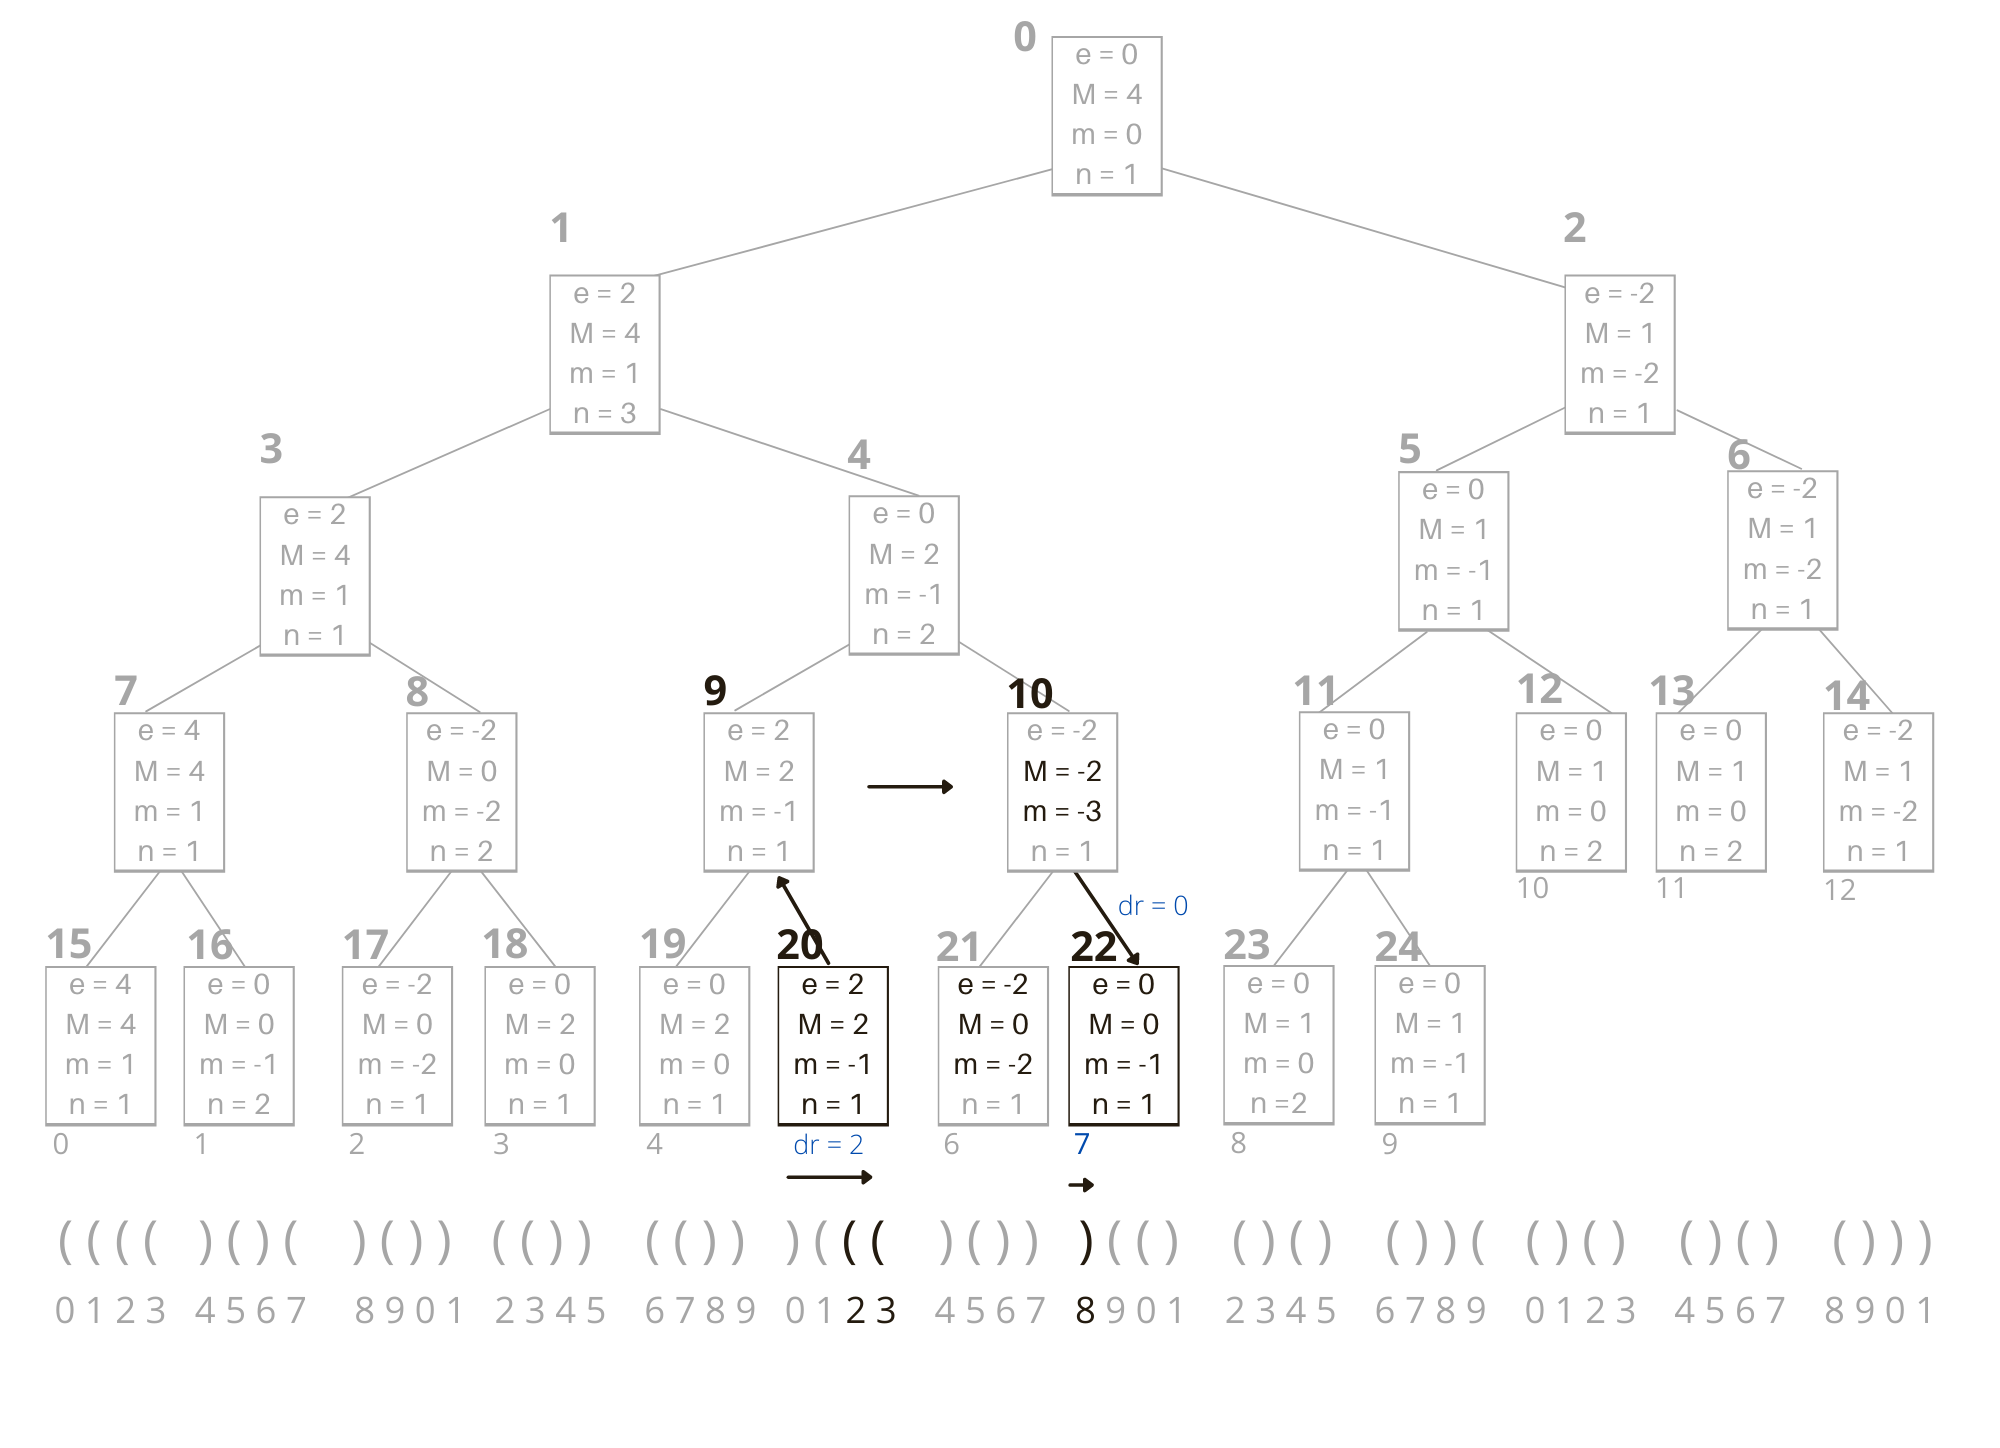
\includegraphics[width=\columnwidth]{images/rmm-tree-bin-fwdsearch.png}
             \label{fig:bin-fwdSearch}
        \end{figure}

        O processo é iniciado através da inspeção dos bits cobertos pelo nó $v=20$, os bits são inspecionados a partir da posição $i+1=22$, até chegar ao
        fim do intervalo deste nó que é $j=23$, durante essa inspeção simulamos a operação de $rank_1$, guardando em uma variável auxiliar $dr$ os valores computados. 
        Ao fim do intervalo, temos que $dr=2$ (como apontado na figura). Como o valor buscado não foi encontrado nessa varredura inicial, precisamos aumentar o nosso espaço de busca, fazemos isso subindo na rmM-tree através dos seus nós. 
        
        \citet{book-compact-data-structures} traz um passo interessante que otimiza a busca na árvore, essa técnica consiste em  verificar se a resposta buscada está no nó à direita do atual,evitando subidas/descidas desnecessárias na rmM-tree. Com base nessa técnica, analisamos o nó à direita de $20$, sem obter sucesso. Atualizamos  $v$ para o índice do seu nó pai $(9)$, e verificamos se os campos do nó à direita (nó $10$) adicionados de $dr$, compreendem o excesso relativo buscado $d$, ou seja $2 -3 \leq 1 \leq -2 +2$. Essa asserção é válida, portanto interrompemos a subida na árvore, e atualizamos o índice guardado em $v$ para $10$, afim de encontrarmos a posição exata onde ocorre o excesso desejado. 
        
        Iniciamos o percurso de descida na árvore. Como buscamos a posição $j$ mais à esquerda possível de $i$, verificamos primeiro se a resposta está contida no intervalo do filho esquerdo do nó $10$, o que não é verdade, em decorrência disso adicionamos à $dr$ o excesso local do nó $21$ ($dr + (-2)= 0$), e descemos então pelo filho direito de $v$, e nesse momento chegamos à um nó folha.
         
         Através desse procedimento de descida na árvore, reduzimos ao máximo o intervalo a ser inspecionado. Iniciamos então a inspeção do intervalo coberto pelo nó $22$, temos que, $dr=-1$ em $BP[28]$, que é o excesso buscado, desse modo temos que a resposta para $fwdSearch(21,-1)$ é $j=28$.
    \end{example}
    
    \begin{algorithm}[htp]
        \SetKwFunction{algo}{algo}
        \SetKwProg{myalg}{Algoritmo}{}{}
        \myalg{fwdBlock(i,d, \&dr)}{
            \Input{Índice a partir do qual começamos a busca, excesso buscado, excesso computado até o momento.}
            \Output{Posição $j$ onde ocorre a resposta, ou $BP.size()$ caso a resposta não exista.}
            \vspace{.3cm}
            $fb \leftarrow \ceil{(i+1)/w}$\\
            $lb \leftarrow \ceil{(i+2)/b} \cdot (b/w)$\\
            \For{$j \leftarrow i+1$ \textbf{to} $(lb\cdot w)-1$}{
                \If{$BP[j]=1$}{$dr \leftarrow dr + 1$}
                \Else{$dr \leftarrow dr -1$}
                \If{$dr = d $}{\Return{$j$}}
            }

            \For{$p \leftarrow fb +1 $ \textbf{to} $lb$}{
                $x \leftarrow bitsRead((p-1) \cdot w)$\\
                \If{$dr + C[x].m \leq d \leq dr + C[x].M$}{\textbf{break}}
                $dr \leftarrow dr + C[x].e$
            }

            \If{$p>lb$}{
                \Return{$lb\cdot b$\tcp{dr não está no bloco subsequente}}
            }
            
            \For{$j \leftarrow (p-1) \cdot w$ \textbf{to} $(p \cdot w)-1$}{
                \If{$BP[j]=1$}{$dr \leftarrow dr + 1$}
                \Else{$dr \leftarrow dr -1$}
                \If{$dr = d $}{\Return{$j$}}
            }
            \Return{$BP.size()$}
        }
        \caption{Busca pelo excesso relativo $d$ em um intervalo de tamanho $b$.}
        \label{alg:fwdBlock}
    \end{algorithm}

    \begin{algorithm}[htp]
        \SetKwFunction{algo}{algo}
        \SetKwProg{myalg}{Algoritmo}{}{}
        \myalg{fwdSearch(i,d)}{
        \Input{Índice a partir do qual a busca deve ser feita, excesso relativo buscado.}
        \Output{Posição $j$ onde ocorre $d$, ou $BP.size()$ caso a resposta não seja encontrada.}
        \vspace{.3cm}
        $dr \leftarrow 0$\\
        $j \leftarrow fwdBlock(i,d,\&dr)$ \tcp{Algoritmo~\ref{alg:fwdBlock}}
        
        \If{$dr = d $}{\Return{$j$}}
        $l \leftarrow \floor{(i+1)/b}$\tcp{l-ésima folha}
        $v \leftarrow leafInTree(l)$\tcp{Algoritmo~\ref{alg:folha-indice}}

        \While{$(v+1)\&(v+2)$ \textbf{and} $dr + R[v+1].m \leq d \leq dr + R[v+1].M$}{
            \If{$v$  mod  $2$}{
                $dr \leftarrow dr + R[v+1].e$
            }
            $v \leftarrow \floor{(v-1)/2}$
        }

        \If{$(v+1)\&(v+2) = 0$}{\Return{$BP.size()$}}

        $v \leftarrow v +1 $\\

        \While{$v < numberLeaves -1 $}{
            $v_l \leftarrow (2 \cdot v)+1$\\
            $v_r \leftarrow v_l + 1$\\
            \If{$dr + R[v_l].m \leq d \leq dr + R[v_l].M$}{
                $v \leftarrow v_l $
            }
            \Else{
                $dr \leftarrow dr + R[v_l].e$\\
                $v \leftarrow v_r$
            }
        }

        $l \leftarrow numLeaf(v)$\tcp{Algoritmo~\ref{alg:folha-indice}}
        $j \leftarrow fwdBlock((l \cdot b)-1,d, \&dr)$\\
        \lIf{$dr = d$ }{\Return{$j$}}
        \lElse{\Return{$BP.size()$}}
        }
        \caption{Busca pela posição onde ocorre um excesso relativo $d$, para um $j>i$}
        \label{alg:fwdSearch-bin}
    \end{algorithm}

\newpage

    \subsection{BwdSearch}\label{sc:bwdsearch}
    Essa operação é bastante similar à \textit{fwdSearch}, portanto não entraremos em tantos detalhes. Além disso, mais à frente fornecemos um exemplo que esclarece o processo para esse tipo de busca. 
    
    O ponto central de \textit{bwdSearch} é que, ao invés de realizarmos uma busca "à frente", como na operação anterior, realizamos uma busca "para trás", assim $bwdSearch$ busca por um índice $j < i$, mais à direita possível, tal que:
    $$bwdsearch(i,d) = max\{j < i | excess(j) = excess(i) - d\}$$

    Como explica \citet{book-compact-data-structures}, a relação acima impacta na nossa busca através da rmM-tree devido aos dados armazenados nas nossas estruturas serem assimétricos, o autor faz então as seguintes considerações relacionadas ao processo de inspeção na rmM-tree,  usando \textit{bwdSearch}:
    \begin{itemize}
        \item Buscamos por um excesso $j<i$, tal que:
         $$excess(j) - excess(i) = - excess(j+1,i) = d,$$ 
         isso faz com que o índice $i$ seja incluído na contagem;
        \item Queremos encontrar um índice $j$ tal que o excesso relativo computado $(dr)$, no intervalo $[i,j]$, seja igual ao excesso buscado, $d$. Mas como $j < i $ e portanto $dr = d = -excess(j+1,i)$, devemos adicionar $1$ unidade à $dr$ ao inspecionarmos um bit codificado como $0$, e diminuir $dr$ em $1$ unidade caso contrário;
        \item  Os valores de excesso são computados a partir de um processo de inspeção de bits da esquerda para a direita. A operação \textit{bwdSearch}, realiza a pesquisa por excesso da direita para a esquerda, isso implica que o excesso buscado $d$, é encontrado em um nó somente quando a asserção $dr - R[v].e + R[v].m \leq d \leq dr - R[v].e + R[v].M$ for válida.
    \end{itemize}
  
    Ademais, como estamos fazendo uma busca por uma posição $j<i$, mais à direita possível, durante o percurso de descida na rmM-tree inspecionamos primeiramente o filho à direita de um nó em busca da resposta, caso não encontremos esta, avançamos no percurso através do filho esquerdo. O Algoritmo~\ref*{alg:bwdSearch-bin} detalha mais sobre esse processo, este algoritmo invoca um método denominado \textit{bwdBlock}, este por usa vez é completamente análogo  ao Algoritmo~\ref{alg:fwdBlock} (a única ressalva é em relação à assimetria discutida acima), portanto não fornecemos aqui o pseudo-código de \textit{bwdBlock}.

  \begin{algorithm}[htp]
        \SetKwFunction{algo}{algo}
        \SetKwProg{myalg}{Algoritmo}{}{}
        \myalg{bwdSearch(i,d)}{
        \Input{Índice $i$ a partir do qual a busca deve ser feita, excesso relativo $d$ desejado}
        \Output{Posição $j$ onde ocorre o $d$, ou $-1$ caso a resposta não seja encontrada}
        \vspace{.3cm}
        $dr \leftarrow 0$\\
        $j \leftarrow bwdBlock(i,d,\&dr)$ \tcp{Análogo ao Algoritmo~\ref{alg:fwdBlock}}
        
        \If{$dr = d $}{\Return{$j$}}
        $l \leftarrow \floor{i/b}$\tcp{l-ésima folha}
        $v \leftarrow leafInTree(l)$\tcp{Algoritmo~\ref{alg:folha-indice}}

        \While{$(v+1)\& v$ \textbf{and} $dr - R[v-1].e + R[v-1].m \leq d \leq dr - R[v-1].e + R[v-1].M$}{
            \If{$v$ mod $2 = 0$}{
                $dr \leftarrow dr - R[v-1].e$
            }
            $v \leftarrow \floor{(v-1)/2}$
        }

        \If{$(v+1)\&v = 0$}{\Return{$-1$}}

        $v \leftarrow v - 1 $\\

        \While{$v < numberLeaves -1 $}{
            $v_l \leftarrow (2 \cdot v)+1$\\
            $v_r \leftarrow v_l + 1$\\
            \If{$dr - R[v_r].e + R[v_r].m \leq d \leq dr - R[v_r].e + R[v_r].M$}{
                $v \leftarrow v_r$
            }
            \Else{
                $dr \leftarrow dr - R[v_r].e$\\
                $v \leftarrow v_l$
            }
        }

        $l \leftarrow numLeaf(v)$\\
        $j \leftarrow bwdBlock(((l+1)\cdot b)-1,d, \&dr)$\\
        \If{$dr = d$ }{\Return{$j$}}
        \Else{\Return{$-1$}}
        }
        \caption{Busca por um excesso relativo $d$, para um $j<i$. }
        \label{alg:bwdSearch-bin}
    \end{algorithm}
    
    \newpage
    O exemplo a seguir, ilustra o processo de busca pelo índice que codifica um nó, cujo parênteses de fechamento é armazenado em $BP[i]$.
    \begin{example}\label{ex:bin-bwd}
        Dado um índice $i$ em $BP$, igual a $50$, encontre o índice $j<i$, mais à direita possível, tal que $excess(j) - excess(i) = 0$


        Como no exemplo anterior, a Figura \ref{fig:bin-bwdSearch}, destaca os bits e índices dos nós inspecionados para chegar a resposta esperada.
        \begin{figure}[h!]
           \centering
             \caption[bwdSearch(50,0).]{Simulação da operação $bwdSearch(50,0)$ em uma rmM-tree binária.}
             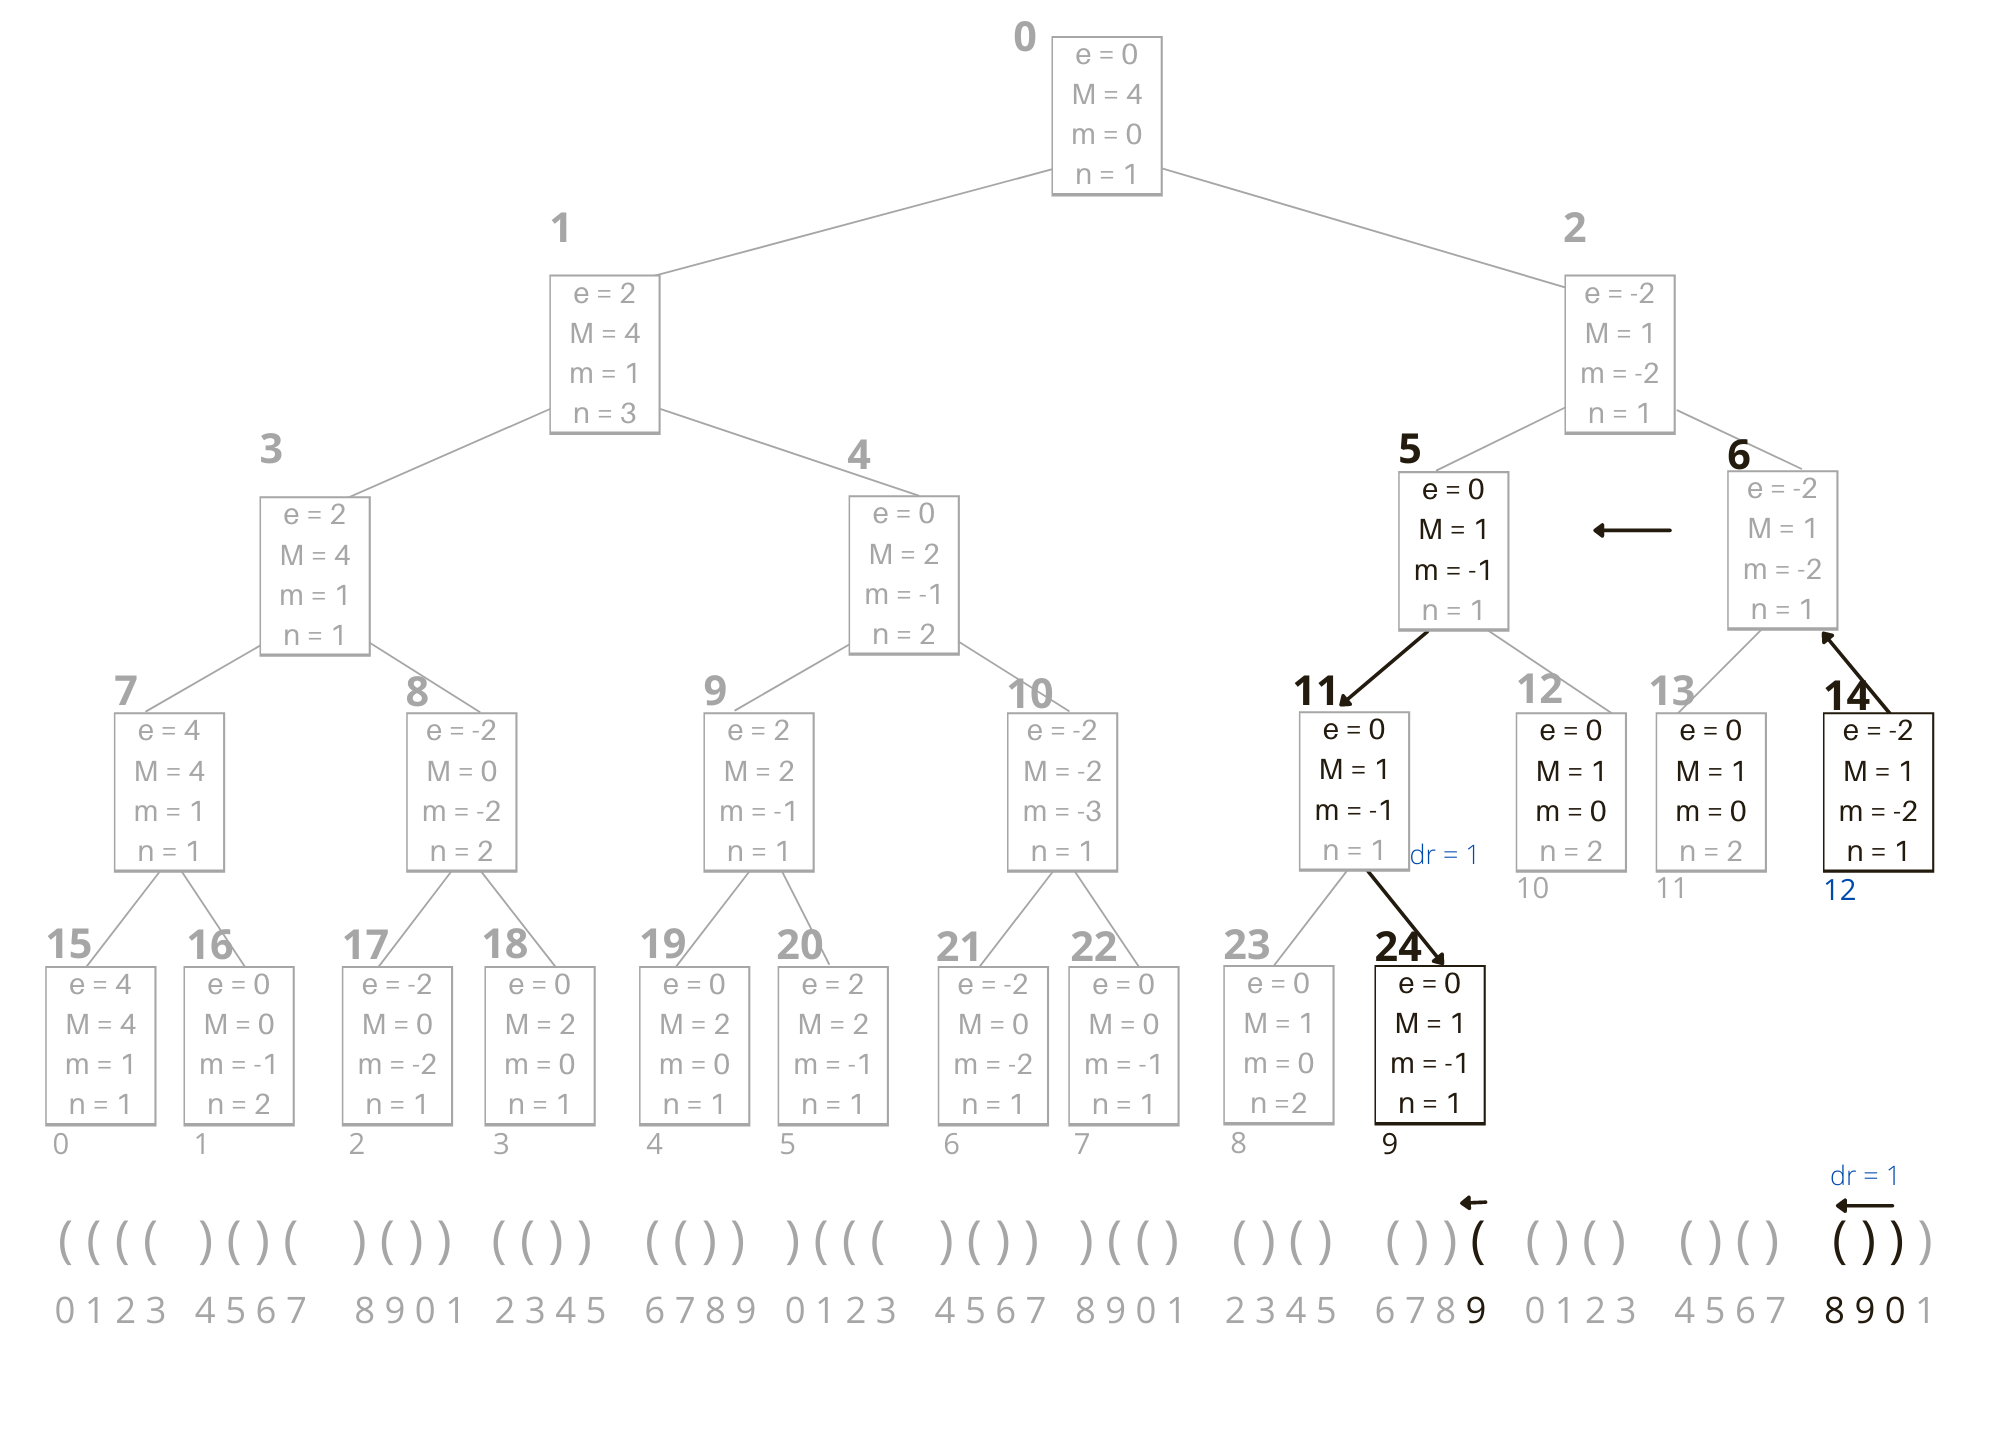
\includegraphics[width=\columnwidth]{images/rmm-tree-bin-bwdsearch.png}
             \label{fig:bin-bwdSearch}
        \end{figure}

        A nossa busca inicia a partir da análise dos bits compreendidos no intervalo da folha $12$ (nó $14$) que compreende o índice $i=50$ (reafirmamos que \textit{bwdSearch} inclui o índice $i$), ao realizarmos a inspeção desta folha, indo de $i=50$ até $j=49$, temos um excesso relativo computado até o momento $(dr)$ igual a $1$. 
        
        Como o excesso é diferente do valor buscado precisamos usar os nós da rmM-tree para encontrar a resposta. Usamos a mesma técnica de otimização de \textit{fwdSearch} e verificamos se $d$ está compreendido nos intervalos de excesso mínimo e máximo do nó à esquerda de $v=14$. A resposta não é encontada no nó $13$, e assim iniciamos o processo de subida na árvore, atualizando o valor de $v$ para $6$.
        
        Analisamos o nó à esquerda de $v=6$, verificando a asserção\footnote{$dr - R[v].e + R[v].m \leq d \leq dr - R[v].e + R[v].m$.} $ 1 -0 -1 \leq 0 \leq 1 -0 +1$. Como a comparação é verdadeira interrompemos o processo de subida na árvore, e atualizamos o valor de $v$ para o nó que contém a resposta.
        
        Iniciamos a descida na árvore, pelo nó $v=5$: verificamos se $d$ está contido nos registros de excesso do filho direito (nó $12$) de $v$, como a busca no filho direito falha, significa que a resposta está no intervalo do filho esquerdo, desse modo atualizamos o índice de $v$ para $11$.

        Continuamos o processo de descida na árvore através do nó $11$, analisamos primeiro o filho direito de $11$ e verificamos que $d$ está contido nos intervalos de excesso deste nó, assim, avançamos para o nó $24$. Como chegamos à um nó folha, interrompemos a busca através dos nós da rmM-tree, e iniciamos uma busca no vetor $BP$. Ao analisarmos o índice $j=39$, $dr$ passa a valer $0$, e portanto a busca pelo excesso $d$ através de \textit{bwdSearch} é concluída, retornando $j=39$. 
    \end{example}




    \subsection{MinExcess}
    Esta é outra importante operação suportada pela rmM-tree. A partir dela podemos obter informações importantes sobre o nosso conjunto de dados, como o menor ancestral comum entre dois nós.
    
    
    O objetivo da \textit{minExcess}, é encontrar o excesso mínimo dentro de um intervalo $[i, j]$. Assim como para as outras operações, esta, inicia-se a partir da inspeção do nó folha que contém o índice $i$. Para \textit{minExcess}, a folha é analisada a partir do índice $i$ até chegarmos ao seu limite, ou até visitarmos o índice $j$, caso este esteja engolobado no intervalo da folha de $i$. 

    Durante a análise da folha, a cada bit lido, guardamos em uma varíavel auxiliar $d$ o valor do excesso relativo computado até o momento, verificamos também se este excesso é o menor até o momento.

    Terminando a inspeção da folha que contém $i$, caso $j$ não esteja contido nela, iniciamos o processo de subida na árvore (caso $j$ esteja contido, a busca é encerrada, e é retornado o menor excesso computado no intervalo analisado). Durante o percurso pela rmM-tree verificamos se os registros de excesso mínimo salvo em cada nó é menor que o excesso mínimo computado até o momento, em caso afirmativo, atualizamos o excesso mínimo computado até o momento. E independente da resposta, atualizamos o valor do excesso relativo $d$.

    Ressalta-se que o percurso em árvore para esta operação é idêntico ao percurso em árvore em \textit{fwdSearch}, sendo interrompido no momento em que estamos prestes a inspecionar um nó $v$, que seja ancestral do nó folha cujo intervalo engloba o índice $j$.

    Para tanto, precisamos de algumas informações, trazidas por \citet{book-compact-data-structures}, que são:
    \begin{itemize}
        \item A profundidade de qualquer nó em $R[v]$ é dada por $\floor{\log (v + 1 )}$;
        \item O pai de um nó, é dado por $\floor{(v-1)/2}$;
        \item À medida que avançamos da esquerda para a direita na rmM-tree, seguindo a abordagem bottom-up, um nó $u$ é dito ancestral de um nó $v$, se a asserção abaixo for válida,
        $$\floor{(v-1)/2^{\floor{\log (v+1)} - \floor{\log (u+1)}}} = u$$
        \item Conforme explica o autor, durante o percurso na árvore, a asserção acima pode ter um comportamento inesperado quando  $u$ for um nó folha, e tiver uma profundidade maior que a do nó alvo (a folha que contém o índice $j$). \citet{book-compact-data-structures} explica que isso pode ocorrer quando o número de folhas não for uma potência de $2$. 
        Para suprir esse problema devemos criar outro critério de continuação de subida na árvore, que é verificar se o índice do nó inspecionado é ou não, maior do que o índice do nó alvo, em caso afirmativo a busca prossegue com a subida na árvore. Desse modo, caso o índice do nó $u$ não for maior do que o índice do nó alvo, e a asserção do tópico anterior for verdadeira, a busca é interrompida.
    \end{itemize}


    Ao encontrarmos o ancestral do nó alvo, interrompemos a subida na rmM-tree, e começamos o processo de descida a partir deste ancestral. O percurso de descida ocorre de modo similar ao da operação \textit{fwdSearch}, verificamos primeiro se o filho  esquerdo do nó visitado é ancestral do nó alvo, em caso positivo descemos na rmM-tree pelo filho esquerdo de $v$.  Em caso negativo, usamos os registros de excesso deste nó para verificar se existe um excesso mínimo menor que o computado até o momento, atualizando esse valor conforme a resposta que obtivermos; e então atualizamos o valor de $v$ para o índice do filho à direita deste nó. 

    Repetimos todo esse processo até que cheguemos a um nó folha. Tendo atingido um nó folha, realizamos a inspeção do mesmo, do início de seu intervalo, até a posição $j$, verificando se os valores de excesso deste intervalo são inferior ao excesso mínimo computado até o momento. Ao término dessa inspeção, temos o excesso mínimo em $BP[i,j]$.


    O exemplo a seguir ilustra como a busca pelo excesso mínimo se dá através da operação \textit{minExcess}.
    \begin{example}
        Dado o intervalo $BP[18,39]$, retornar o menor excesso.

       \begin{figure}[!ht]
           \centering
             \caption[minExcess(18,39).]{Simulação da operação $minExcess(18,39)$ em uma rmM-tree binária.}
             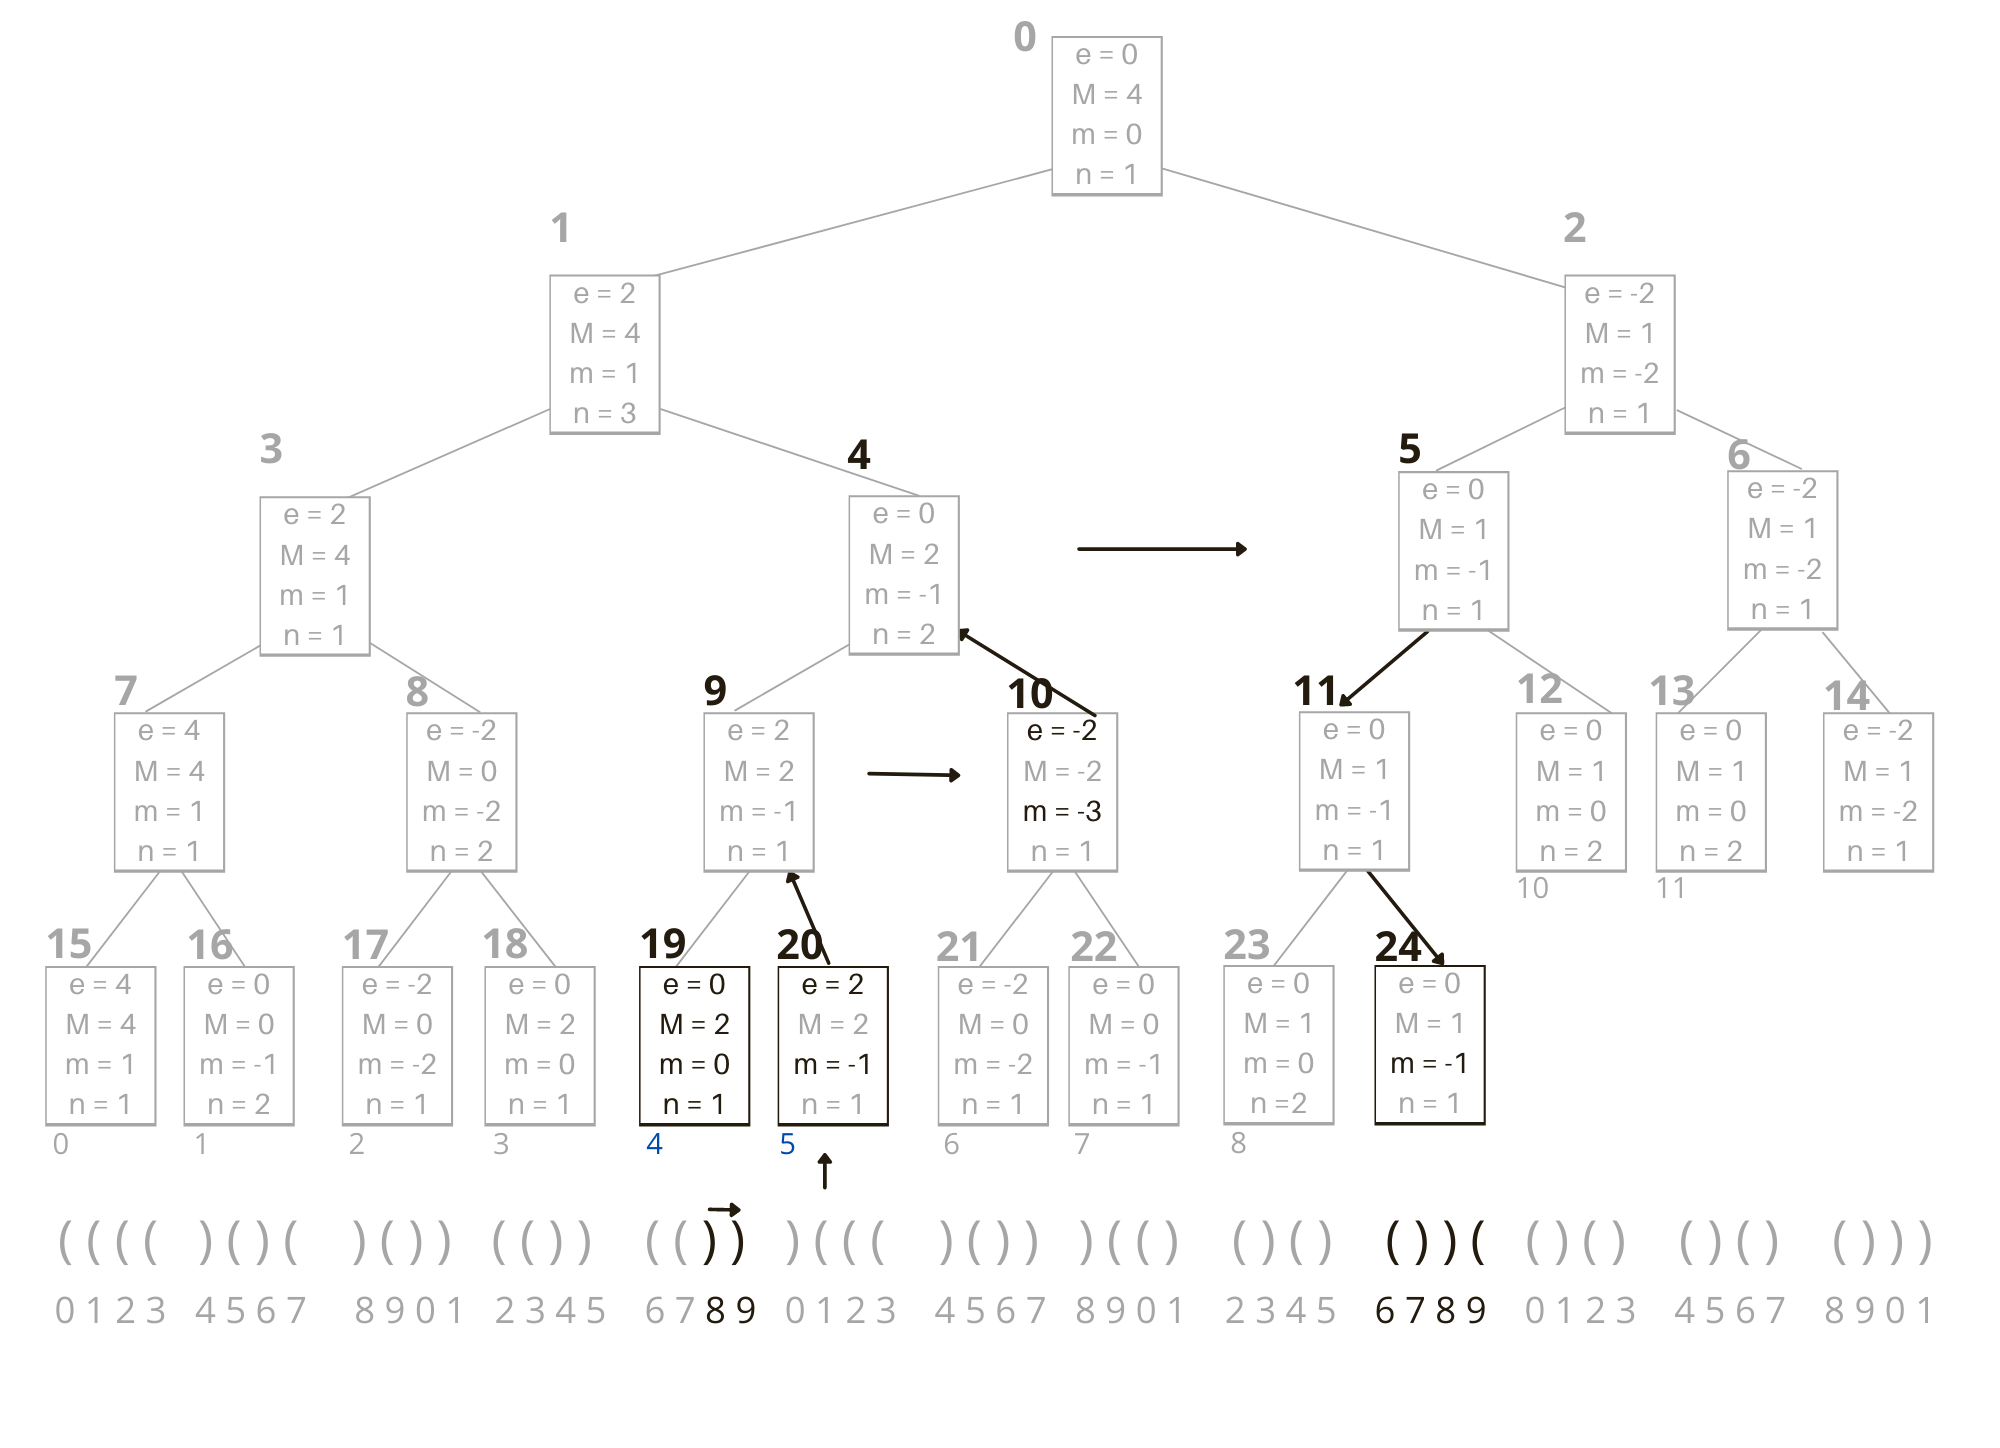
\includegraphics[width=\columnwidth]{images/rmm-tree-bin-minexcess.png}
             \label{fig:bin-minexcess}
        \end{figure}

        Primeiro fazemos a análise da folha que contém o índice $i$, realizamos uma varredura parcial do intervalo da folha $4$ (nó $19$), indo de $i=18$ até $p=19$, nesse momento temos que o excesso mínimo ($m$) e o excesso local ($d$) computado até o momento, valem $-2$.

        Como $j$ não está compreendido no intervalo da folha $4$, precisamos identificar o nó folha cujo o intervalo compreende $j$, este nó é dado por $x=24$. Verificamos se o excesso mínimo no nó à direita de $v=19$, é menor que o excesso computado até o momento, como a asserção é válida $-2 -1 < -2$ (por $d + R[20].m < d]$), atualizamos o valor de $m$ para $-3$, e o valor de $d$ para $0$.

        Como $j$ não está compreendido no irmão à direita de $v$, iniciamos o percurso de subida na árvore através nó $9$. Analisamos se o nó à direita de $v$ é ancestral do nó alvo, e obtivemos que o nó $10$ não é ancestral de $x$, com base nos registros do nó $10$ atualizamos o valor de $d$ para $-2$, e subimos na árvore através do nó $4$. Novamente, verificamos se o nó à direita ($5$) do nó atual é ancestral do nó $x=24$, e nesse momento
        temos uma afirmação verdadeira. 
        
        Tendo achado o nó ancestral de $x$, interrompemos o processo de subida na árvore, e iniciamos o processo de descida  a partir do nó $v=5$. Ao analisarmos os filhos de $v$, temos que o seu filho esquerdo (nó $11$) é ancestral do nó $24$, então atualizamos o valor de $v$ para $11$, e verificamos os filhos do mesmo. Temos nesse momento que o filho esquerdo de $v$ (nó $23$) não é ancestral do nó alvo, desse modo atualizamos o valor de $v$, para o índice do seu filho à direita, que é o próprio nó alvo.

        Como chegamos à um nó folha, interropemos a verificação dos nós da rmM-tree, e iniciamos a verificação do excesso mínimo na folha $9$ (nó $24$), ao pecorrer está folha o valor do excesso mínimo computado até o momento não é alterado, e portanto $BP[18,39].m=-3$.
    \end{example}

        
        Uma outra variação dessa operação é a \textit{maxExcess}, o processo para responder esta é completamente análogo ao descrito acima, mudando apenas os registros da rmM-tree analisados (ao invés de verificarmos o excesso mínimo, verificamos o excesso máximo).

    \subsection{MinCount e MinSelectExcess}
    \textit{MinCount e MinSelectExcess} possuem um alto nível de similaridade entre si, e também são análogas à \textit{minExcess}, portanto não entraremos nos detalhes de implementação das duas.
    
    De modo geral, o objetivo da operação \textit{minCount} é computar o número de vezes que o excesso mínimo aparece no intervalo $BP[i,j]$, ao passo que a operação \textit{minSelectExcess}, 
    objetiva encontrar o índice dentro do intervalo $[i,j]$, onde ocorre a $t-$ésima ocorrência do excesso mínimo computado neste mesmo intervalo. 
    Observe que para ambas as operações, é necessário primeiro computar o excesso mínimo dentro do intervalo fornecido, para tanto, podemos fazer uma chamada a função \textit{minExcess}, 
    e então pecorrer a rmM-tree em busca da resposta esperada para cada operação. 
    
    Para realizar a operação \textit{minCount}, cria-se um acumulador que é incrementado através do registro $n$ da rmM-tree, sempre que passarmos por um nó cujo o valor de excesso mínimo for igual ao excesso computado por \textit{minExcess}. 

    A operação \textit{minSelectExcess} é análoga, para ela, pode-se criar um acumulador que recebe o valor $t$, passado para a função, e assim ao visitar um nó cujo o valor de excesso mínimo é igual ao valor computado por \textit{minExcess}, subtraímos do acumulador  o valor armazenado em $n$, a resposta nesse caso é encontrada quando o acumulador atinge a marca menor ou igual a $0$. Para ambas as operações, o processo de subida e descida na árvore se dá de igual modo ao mostrado em \textit{minExcess}.


    Essas são as únicas operações que usam o registro $n$ da rmM-tree, portanto não há necessidade de fazer a computação deste, caso o objetivo da sua estrutura não englobe uma destas operações ou suas derivadas.

    \subsection{Derivadas}
    Esta seção demonstra como diversas operações sobre a rmM-tree podem ser escritas de modo eficiente a partir das operações descritas anteriormente.

    \begin{itemize}
        \item \textbf{rmq(i,j)}: busca pela primeira posição onde ocorre o excesso mínimo computado dentro do intervalo  $BP[i,j]$. Ou seja:
            $$rmq(i,j) =\min \{ \argmin\{excess(p) | i \leq p \leq j\}\} $$
    
        Para responder esta operação, podemos computar primeiro o exesso mínimo dentro do intervalo $[i,j]$, e em seguida realizar uma busca a partir de $i$, pela posição $j$ onde ocorre o excesso computado.
        Temos assim:
        $$rmq(i,j) = fwdSearch(i-1,minExcess(i,j))$$
        Repare que o primeiro parâmetro  em \textit{fwdSearch} é subtraído em $1$, isso acontece porque o intervalo da busca  de \textit{fwdSearch} é aberto, ou seja, não incluí o índice passado nas buscas, ao passo que o intervalo de \textit{rmq} é fechado, incluindo $i$ e  $j$ nas buscas. 
    
        \item \textbf{rMq(i,j)}: similar a operação anterior, \textit{rMq}, busca a posição mais à esquerda de $i$ onde ocorre o excesso máximo computado em $[i,j]$. Ou seja:
        $$rMq(i,j) =\max\{ \argmax\{excess(p) | i \leq p \leq j\}\} $$   
        
        Assim:
            $$rMq(i,j) = fwdSearch(i-1, maxExcess(i,j))$$


        \item \textbf{findClose(i)}: essa operação recebe como parâmetro um índice $i$, correspondente à um nó, isto é, à um parênteses de abertura, e a partir da operação \textit{fwdSearch} busca o parênteses de fechamento correspondente. \\
        A operação \textit{fwdSearch} pecorre o vetor de bits e a rmM-tree a partir de $i+1$ até que encontre o índice $j > i $, tal que a profundidade do elemento codificado em $j$ (em relação à $i$) seja $-1$, ou seja, $excess(j) - excess(i+1) = -1 $.  Assim:
        $$findClose(i) = fwdSearch(i,-1)$$
            
        \item \textbf{findOpen(i)}:  seja $BP[i]=0$, \textit{findOpen}, faz uma busca por um $j < i $ tal que $excess(j) - excess(i) = 0$ e $excess(j)+1=1$. 
        Isso nos dá:
        $$findOpen(i) = bwdSearch(i,0)+1$$
        
        \item \textbf{enclose(i)}: dado um índice $i$, que indica a codificação de um nó $x$, \textit{enclose} retornará o índice do parênteses mais envolvente de $x$, ou seja, o pai do nó $x$. Essa operação faz o uso de \textit{bwdSearch} para encontrar a posição $j<i$, mais à direita de $i$, tal que $excess(j) - 2 = 1$. Ou seja:
        $$enclose(i) = bwdSearch(i,-2) + 1$$

        \item  \textbf{levelAncestor(i,d)}: essa operação buscará pelo nó $x$ que seja ancestral e esteja $d$ níveis acima de um nó $i$. Para tanto podemos usar a operação \textit{bwdSearch}. Por questões de simetria, já discutidas anteriormente, devemos passar o valor de $d$ como negativo em \textit{bwdSearch}, e assim temos:
        $$levelAncestor(i,d) = bwdSearch(i,-d-1)+1$$
        
        \item \textbf{isAncestor(x,y)}: essa função tem por objetivo verificar se um nó $x$ é ancestral de um nó $y$, para tanto, basta verificar se $y$ está contido na hierarquia de $x$. Podemos usar \textit{findClose}, como mostrado abaixo:
        $$ isAncestor(x,y) = (x < y  \mbox{ and }  y < findClose(x))$$
        
        \item \textbf{parent(i)}: dado o elemento $BP[i]=1$, \textit{parent} busca através de \textit{enclose} o índice do nó que codifica
        o pai do nó $i$:
        $$parent(i) = enclose(i)$$
        
        \item \textbf{lca(i,j)}: busca o menor ancestral comum entre dois nós, codificados nos índices $i$ e $j$. Existem 3 possibilidades de retorno para \textit{lca}, são eles:
        $$lca(i,j) =
               \begin{cases}
                     i,  \mbox{se } isancestor(i,j); \\
                    j, \mbox{se } isancestor(j,i); \\
                    parent(rmq(i ,j)+1)
               \end{cases}
        $$

        \item \textbf{deepestNode(i)}: dado o nó  $BP[i]$, \textit{deepestNode} retorna o descendente com maior profundidade deste nó (localizado mais à esquerda possível). Para calcular o maior excesso possível a partir de $i$ podemos usar a operação \textit{maxExcess}. Como esse excesso deve estar limitado ao escopo do nó codificado em $i$, temos a seguinte relação:

        $$deepestNode(i) = rMq(i, findClose(i))$$

        A operação $rMq$ é usada aqui para invocar \textit{maxExcess} e em seguida retornar a posição exata onde ocorre o excesso computado, que indica o índice do nó procurado.

        \item \textbf{degree(i)}: esta operação contabiliza o número de filhos de um nó codificado em $i$. Como a sequência que representa a nossa ávore de entrada é balanceada, temos que dentro do intervalo (aberto) de hierarquia de um nó, atingimos o excesso mínimo sempre que finalizamos a codificação de um de seus nós filhos. Levando isso em consideração, podemos calcular \textit{degree} do seguinte modo:
        $$degree(i) = minCount(i+1, findClose(i)-1)$$
        
        \item \textbf{childRank(i)}: dado um índice $i$, \textit{childRank}, contabiliza o número de irmãos que o nó codificado em $i$ possui à sua esquerda. Tendo as operações definidas anteriormente, podemos responder \textit{childRank} conforme mostrado abaixo:
        $$
               childRank(i) = minCount(parent(i)+1, i) +1
        $$
        
        \item \textbf{nextSibling(i)}: dado um nó codificado em $i$, \textit{nextSibling} busca pelo irmão do nó $i$, codificado em $j$, tal que $j>i$.
        $$nextSibling(i) = findClose(i) +1$$
        
        \item \textbf{prevSibling(i)}: análoga a \textit{nextSibling}, esta operação busca pelo irmão imediatamente à esquerda do nó codificado por $i$. Ou seja:
        $$prevSibling(i) = findOpen(i-1)$$
        
        \item \textbf{child(i,t)}: dado um índice $i$ que codifica um nó, \textit{child} calcula a posição em $BP$ onde ocorre a codificação do $t$-ésimo filho de $i$  -- ou seja a posição $j$ onde acontece a $t$-ésima ocorrência do excesso mínimo dentro da hierarquia do nó analisado --  desse modo, podemos escrever
        \textit{child} em função de \textit{findClose} e \text{minSelectExcess}:
        $$p = findClose(i)$$
        $$child(i,t) = minSelectExcess(i+1,p-1,t-1) + 1 $$

        \item \textbf{lastChild(i)}: busca pelo último filho de um nó codificado em $BP[i]$:
        $$lastChild(i) = findOpen(findClose(i)-1)$$
        
        \item  \textbf{subtreeSize(i)}: calcula o tamanho da subárvore enraízada no nó $i$, para tanto, basta realizar uma contagem dos nós codificados no intervalo de contenção de $i$, ou seja:
        $$subtreeSize(i)= \floor{(findClose(i) - i + 1)/2}$$
        
        \item \textbf{levelNext(i)}: busca o nó a direita do nó codificado por $i$, em seu mesmo nível:
        $$levelNext(i) = fwdSearch(findClose(i),1)$$
        
        \item \textbf{levelPrev(i)}: análoga a \textit{levelNext}, esta função busca pelo primeiro nó imediatamente à esquerda do nó codificado em $i$ e que possui a mesma profundidade deste. Como este caso trata de uma busca à esquerda de um índice, usamos \textit{bwdSearch} para realizar esta operação:
        $$levelPrev(i) = findOpen(bwdSearch(i,0)+1)$$
        
        \item \textbf{levelLeftMost(d)}: busca pelo nó mais à esquerda da raíz, com profundidade $d$, assim:
        $$levelLeftMost(d) = fwdSearch(0,d-1)$$
        
        \item \textbf{levelRightMost}: usando como referência a raíz, busca pelo nó mais à direita, cuja profundidade é igual  à $d$:
        $$levelRightMost(d) = findOpen(bwdSearch(BP.size()-1,d)+1)$$
    \end{itemize}
    
    Algumas das operações a seguir, usam em seu escopo as operações listadas acima e as operações suportadas pela estrutura de vetores de bits (algumas, como o caso de \textit{depth} usam apenas estas últimas). Isto evidencia a importância do cuidado ao escolhermos estruturas de suporte apropriadas, afim de acelerar nossas operações.
        \begin{itemize}
            \item \textbf{firstChild(i)}: retorna o primeiro filho do nó codificado por $i$, logo:
            $$firstChild(i) = i +1$$
            \item \textbf{isLeaf(i)}: dado um nó codificado em $i$, verifica se este é um nó folha, essa é uma das operações mais simples suportadas pela \textit{rmM-tree}, necessistando apenas de 2 comparações, veja abaixo:
            $$isLeaf(i) = (BP[i] = 1 \land BP[i+1]=0)$$
            \item \textbf{depth(i)}: computa a profundidade de um nó codificado por $i$, para tanto basta verificar o exesso em $BP[0,i]$, ou seja:
            $$depth(i) = excess(i)$$
            \item \textbf{leafRank(i)}: contabiliza a quantidade de folhas existentes em um intervalo que vai de $0$ à $i$. Em nossa implementação, usamos a operação \textit{rank},
            suportada pela estrutura de vetores de bits, para fornecer suporte à esta. Assim, basta buscar a quantidade de ocorrêncas de bits $1$ seguidos por um bit $0$.
            $$leafRank(i) = rank_{10}(i)$$
            \item \textbf{leafSelect(i)}: esta operação nos permite buscar pela $i-$ésima folha em $BP$, para tanto é necessário procurar pela $i-$ésima ocorrência do padrão $10$:
            $$leafSelect(i) = select_{10}(i)$$
            \item \textbf{leftMostLeaf(i)}: retorna a folha mais à esquerda da subárvore com raíz em $i$.
            $$leftMostLeaf(i) = leafSelect(leafRank(i-1)+1)$$
            \item  \textbf{rightMostLeaf(i)}: retorna a folha mais à direita da subárvore com raíz em $i$.
            $$rightMostLeaf(i) = leafSelect(leafRank(findClose(i)))$$
            \item \textbf{preRank(i)}: retorna o índice do nó da árvore de entrada correspondente à $BP[i]$,  considerando um percurso pré-ordem.
            $$preRank(i) = rank_1(i)$$
            \item \textbf{postRank(i)}: análoga à \textit{preRanj}, esta operação leva em consideração um percurso pós-ordem.
            $$postRank(i) = rank_0(findClose(i))$$
            \item \textbf{preSelect(i)}: retorna a posição em $BP$ correspondente ao $i$-ésimo nó da árvore de entrada, considerando um percurso em pré-ordem:
            $$preSelect(i) = select_1(i)$$
            \item \textbf{postSelect}: retorna a posição em $BP$ correspondente ao $i$-ésimo nó da árvore de entrada, considerando um percurso em pós-ordem:
            $$postSelect(i) = findOpen(select_0(i))$$
        \end{itemize} 

\begin{table}[h!]
	\centering
	\caption[Operações sobre a RMM-tree clássica]{Operações suportadas pela rmM-tree bináriaW}
	\label{tbl:classicOperations-rmm-tree}
	\rowcolors{2}{lightgray!30}{white}
	\resizebox{\columnwidth}{!}{
	\begin{tabular}{ll}
	\toprule
	\textbf{Operação} & \textbf{Retorno} \\
	\toprule
    
	fwdSearch(i,d)  & Índice $j$, tal que $excess(j) = excess(i) + d$\\
	bwdSearch(i,d)  & Índice $j$, tal que $excess(j+1,i) = -d$\\
	minExcess(i,j) / maxExcess(i,j)  & Excesso mínimo/máximo em $i,j$\\
	minCount(i,j)  & Número de vezes que o excesso mínimo aparece em $i,j$\\
	minSelectExcess(i,j,t)  & Índice da $t-$ésima ocorrência do excesso mínimo em um intervalo\\
	enclose(i) & Posição do parênteses de abertura que envolve  $BV[i]$  \\
	rmq(i,j) / rMq(i,j) & $p>=i$ mais à esquerda de $i$, onde ocorre o excesso mínimo/máximo do intervalo dado \\
	rank$_1$(i) / rank$_0$(i) & Número de parênteses abrindo/fechando em $BV[0,i]$ \\
    select$_1$(i) / select$_0$(i) & Posição do i-ésimo parênteses de abertura/fechamento\\
    preRank(i)/postRank(i) & rank de $i$ calculado a partir de um percurso \textit{preorder \mbox{ ou } postorder} \\
    preSelect(i)/postSelect(i) & retorna o nó com \textit{preorder/postorder} $i$\\
    isLeaf(i) & Verifica se $BV[i]$ codifica uma folha \\
    isAncestor(i,j) & Verifica se o nó codificado em $i$ é ancestral de $j$ \\
    depth(i) & Profundidade do nó $i$ \\
    parent(i) & Obtém o pai do nó $i$ \\
    firstChild(i) / lastChild(i) & Retorna o primeiro/último filho do nó codficiado em $BV[i]$ \\
    child(i,t)&$t-$ésimo filho do nó codificado em $i$\\
    nextSibling(i) / prevSibling(i) & Primeiro irmão à direita/esquerda de $i$ \\
    subtreeSize(i) & Número de nós enraízados na subárvore de $i$ \\
    levelAncestor(i,d) & Ancestral $j$ de $i$ tal que $depth(j) = depth(i) - d$\\
    levelNext(i) / levelPrev(i) & Nó à direita/esquerda de $i$ com a mesma profundidade de $i$.\\
    levelLeftMost(d) / levelRightMost(d) &Nó mais à esquerda/direita, com profundidade d.\\
    lca(i,j)&Menor ancestral comum dos nós codificados em $i$ e $j$\\
    deepestNode(i)&Nó mais profundo de $i$ (mais à direita possível)\\
    degree(i)&Número de filhos do nó $i$ \\
    childRank(i)&Número de irmãos à esquerda do nó codificado em $i$\\
    leafRank(i)& Número de folhas à esquerda da folha codificada em $i$ \\
    leafSelect(i)& $i-$ésima folha em $BV[0,size-1]$ \\
    leftMostLeaf(i)& folha codificada em $j$, mais à direita de $i$, tal que $j<i$\\
    rightMostLeaf(i)& folha codificada em $j$, mais à direita possível, tal que $j \leq i$\\
	\bottomrule
	\end{tabular}
	}
\end{table}



\section{Estruturas de dados Cache-sensitive}\label{sec:cache-sensitive}
%A redução do preço e o aumento da capacidade da memória principal possibilitam que grandes conjuntos de dados residam na memória principal \citet{paper-effect-node-size-cache-b-trees},
%onde o tempo para acessar um dado é menor. 

Como vimos, o uso das estruturas de dados sucintas permitem que grandes conjuntos de dados residam e sejam operados na memória principal.  \citet{paper-effect-node-size-cache-b-trees} nos mostram que, com os  dados residindo na memória RAM, um novo gargalo é criado, que surge em decorrência do atraso ao buscarmos na memória principal um dado que não se encontra em cache. 

Quando uma referência de memória é satisfeita pela cache, estas prosseguem na velocidade do processador, as referências não satisfeitas incorrem em uma penalidade no tempo de execução da busca, devido a necessidade de buscar o bloco correspondente na memória principal. Conforme citam \citet{paper-effect-node-size-cache-b-trees} o tempo gasto para buscar um dado em cache é de uma à duas ordens de magnitude menor do que a latência para a recuperação de dados na memória principal. Desse modo, a utilização inadequada da cache pode fazer com que a latência da memória se torne um gargalo crescente de desempenho, impedindo que as aplicações se beneficiem das crescentes melhorias de hardware \citep{paper-making-btree-cache}.
 
\citet{paper-effect-node-size-cache-b-trees} realizaram um estudo sobre o efeito da maximização da quantidade de informações relevantes armazenada em um nó de uma árvore denominada \textit{Cache-Sensitive Search Trees (CSS-tree)}, uma estrutura de índice consciente de cache, que possui um desempenho em realização de pesquisas superior ao da pesquisa binária \citep{paper-making-btree-cache}. De acordo com os autores o custo de execução de uma pesquisa é baseado em quatro fatores: número de instruções $(I)$, quantidade de \textit{cache misses} $(CM)$, número de previsão  erradas de ramificação $(R)$ e número de erros de TLB \footnote{ Translation Lookaside Buffer  - armazena as entradas das tabelas de páginas da memória usadas recentemente}  $(T)$ \citep{paper-effect-node-size-cache-b-trees}.  Esse tempo é modelado pela equação abaixo,

\begin{eqnarray*}
    t = (I \cdot cpi) + (CM \cdot miss\_latency) + (R \cdot pred\_penalty) + (T \cdot tlb\_penalty) 
\end{eqnarray*}

sendo:

\begin{itemize}
    \item $t$ o tempo total de execução em ciclos de clock;
    \item $cpi$: custo de execução por instrução;
    \item $miss\_latency$:  tempo acrescido em decorrência de uma falta de cache;
    \item $pred\_penalty$: custo de pecorrer um ramo na árvore sem encontrar resposta, e
    \item $tlb\_penalty$: custo para recuperar uma entrada na  tabela de páginas.
\end{itemize}

Além disso \citet{paper-effect-node-size-cache-b-trees} nos mostram que o número de perdas de cache é limitado pela altura  da árvore,  essa por sua vez está diretamente relacionada ao número de nós folhas, e ao fator de ramificação da árvore. Com base nisso, parte da estratégia dos autores consistiu em aumentar a quantidade de dados coberto por nó folha, visando minimizar quantidade de folhas, consequentemente a altura da árvore, fazendo assim um melhor aproveitamento de uma linha de cache\footnote{Unidade básica de transferência entre cache e memória RAM}. 
 
Os resultados do trabalho citado nos mostram que, ao escolhermos um número de entradas adequado para um nó (não ultrapassando o tamanho de uma linha de cache), temos um número de \textit{cache misses} minimizado.  Além disso, os resultados experimentais de \citet{paper-effect-node-size-cache-b-trees}  revelam que, mesmo ao maximizar o tamanho de um nó, ao ponto de ultrapassar o tamanho de uma linha de cache, a quantidade de informações presentes nos nós fazem com que o número de instruções e de previsões erradas, assim como a quantidade de páginas $TLB$, reduza de modo tão drástico que compensam a quantidade de falhas de cache, superando o desempenho da \textit{CSS-tree} com tamanho de nó menor.

 \citet{paper-making-btree-cache} também fizeram um estudo sobre o impacto de diferentes versões da \textit{CSS-tree} em cache, o objetivo deles era melhorar o desempenho das operações de atualização suportadas pela \text{CSS-tree}. Com base nisto, os autores propuseram uma estrutura baseada em árvores $B^+$ -- tendo em vista que estas possuem excelente desempenho para conjuntos de dados que requerem atualizações incrementais-- denominada  \textit{Cache Sensitive $B^+$-tree (CSB$^+$-tree)}.

 No total, \citet{paper-making-btree-cache} criaram $3$ versões da \textit{CSS-tree}, são elas: \textit{CSB$^+$-tree, CSB$^+$-tree segmentada} e  \textit{Full CSB$^+$-tree}, estas se diferenciam em quantidade de ramificações, capacidade de armazenamento de nó, e contiguidade de nós. Os resultados experimentais do estudo revelaram que: todas as versões da \textit{CSB$^+$-tree} possuem desempenho superior ao da \textit{B$^+$-tree}, tanto para pesquisa quanto para atualização, devido ao maior fator de ramificação das \textit{CSB$^+$-tree}. Como esperado pelos autores, as \textit{CSS-tree}, apresentam desempenho superior ao das \textit{CSB$^+$-tree} para operações de pesquisa, isso se deve também ao elevado fator de ramificação da estrutura clássica se comparado aos das diferentes versões da \textit{CSB$^+$-tree}. Em relação as $3$ versões da \textit{CSB$^+$-tree}, obtiveram melhor desempenho nas operações de pesquisa, àquelas que possuíam maior fator de ramificação. Por fim, as \textit{CSB$^+$-tree} apresentaram, conforme o objetivo do trabalho, melhor desempenho nas operações de atualização frente à \textit{CSS-tree} devido a quantidade de informações presentes nos nós da árvore\citep{paper-making-btree-cache}.

Com base no exposto acima, e levando em consideração que a range min-Max tree possui baixo fator de ramificação e baixo aproveitamento de linha de cache. Propomos uma versão alternativa da rmM-tree, a rmM-tree k-ária. Nosso objetivo com essa estrutura é  realizar um melhor aproveitamento da cache, com base no princípio de localidade espacial, maximizando a quantidade de dados transferidos entre níveis e aumentando o fator de ramificação dessa estrutura, essa proposta é melhor detalhada no próximo capítulo.
%\citet{paper-making-btree-cache} usam o mesmo príncipio do alto fator de ramificação das árvores B e seu melhor aproveitamento de cache em relação às árvores binárias para construir 
%uma variação de Árvores Sensíveis a Cache (CSS-Tree). Os autores usaram uma variação das árvores B+ que armazena os seus nós de forma contígua (possiblitando assim o armazenamento apenas 
%do endereço do primeiro filho em um nó), maximizando assim  o espaço de armazenamento dos índices, e em decorrência disso diminuindo ainda mais o fator de ramificação. Os resultados experimentais 
%deste trabalho, mostraram 

